\chapter{Empirical Study on the Cast Operator}
\label{cha:casts}

The main goal of a \emph{static} type system
is to prevent certain kinds of errors from happening at run time.
A type system is formulated as a set of constraints that gives any expression or term in a program a well-defined type.
Any program not satisfying the constraints specified by the type system is
simply rejected by the compiler.

Nevertheless, often a static type system is insufficiently precise.
The type checker is necessarily conservative:
it must not accept invalid programs,
but it may reject programs that are valid but whose validity cannot be ensured at compile time.
However, there are situations when the developer has more information
about the program than can be encoded---or encoded easily---into the types.
To that end, programming languages often provide mechanisms to make the typing constraints less strict,
allowing more valid programs at the expense of more errors at run time.

A common mechanism for relaxing the static typing constraints in object-oriented languages is \emph{casting}.
In programming languages with subtyping---or \emph{subtype polymorphism}~\citep{cardelliUnderstandingTypesData1985}---such as \java{}, \csharp{} or \cpp{},
casting allows an expression to be viewed at a different type than the one at which it was defined.
Casts are checked dynamically, \ie, at run-time, to ensure that the object
being cast is an instance of the desired type.

We aim to understand why developers use casts.
Why is the static type system insufficient,
requiring an escape hatch into dynamic type checking?
Specifically, we attempt to answer the following three research questions:

\begin{enumerate}[label=$RQ/C\arabic*:$,ref=$RQ/C\arabic*$,leftmargin=3.4\parindent]
\item\label{casts:rq1}{\bf \crqA} \crqAdesc{}
\item\label{casts:rq2}{\bf \crqB} \crqBdesc{}
\item\label{casts:rq3}{\bf \crqC} \crqCdesc{}
\end{enumerate}

To answer these research questions, we devise
\emph{usage patterns}.
Usage patterns are \emph{recurrent programming idioms} used by developers to solve a specific issue.
Usage patterns enable the categorization of different kinds of cast usages and
thus provide insights into how the language is being used by developers in real-world applications.
Our cast usage patterns can be:
\begin{inparaenum}[(1)]
\item a reference for current and future language designers
to make more informed decisions about programming languages,
\eg{},
the addition of \emph{smart casts} in \lang{Kotlin},\footnote{\url{https://kotlinlang.org/docs/reference/typecasts.html\#smart-casts}}
\item a reference for tool builders, \eg{}, by providing more precise or new
  refactoring or code smell analyses,
\item a guide for researchers to test new language features, \eg{},~\cite{wintherGuardedTypePromotion2011} or to carry out controlled
  experiments about programming, \eg{},~\cite{stuchlikStaticVsDynamic2011}, and
\item a guide for developers for best or better practices.
\end{inparaenum}
To answer our research questions,
we empirically study how casts are used by developers.
The results of this study have been submitted for publication to \conf{OOPSLA}{19}.


\section*{Outline}

Section~\ref{sec:casts:background} provides an introduction to casts in \java{},
while Section~\ref{sec:casts:issues} illustrates the sort of problems developers have when applying casting conversions.
In Section~\ref{sec:casts:methodology} we introduce the methodology we used to analyse casts and to devise cast usage patterns.
Sections~\ref{sec:casts:overview} and~\ref{sec:casts:patterns} present the cast usage patterns and answers our research questions.
Finally, Section~\ref{sec:casts:discussion} discusses the patterns we found,
while Section~\ref{sec:casts:conclusions} concludes.

\newcommand{\npattern}{31}
\newcommand{\ngroup}{10}
\newcommand{\nprim}{250}
\newcommand{\nbrokenlinks}{221}


\section{Casts in \java{}}
\label{sec:casts:background}

While casts should be familiar to most developers of object-oriented languages,
because they have different semantics in different programming languages,
we briefly summarize the meaning of casts in \java{} and the terminology used in the rest of this chapter.

In object-oriented programming languages like \java{},
the subtype mechanism allows the interoperability of two different but related types.
As~\cite{pierceTypesProgrammingLanguages2002} states,
``[\ldots] $S$ is a subtype of $T$, written $S <: T$,
to mean that any term of type $S$ can safely be used in a context where a term of type $T$ is expected.
This view of subtyping is often called the \emph{principle of safe substitution}''~\citep{liskovBehavioralNotionSubtyping1994}.
Conversely, if $S$ is a subtype of $T$, we say that $T$ is a supertype of $S$.

A cast operation, written \code{(T) e} in \java{}
consists of a \emph{target type} \code{T} and an \emph{operand} \code{e}.
The operand evaluates to a \emph{source value} which has a run-time
\emph{source type}.
In \java{}, a source reference type is always a class type.
For a particular cast evaluated at run time, 
the \emph{source} of the cast is the expression in the program that
created the source value.
For reference casts, the source is an object allocation.
The source may or may not be known statically.

An \emph{upcast} occurs when the cast is from a source reference type $S$ to a target reference type $T$,
where $T$ is a supertype of $S$.
In our terminology, upcasts include identity casts where the target type
is the same as the type of the operand.
An upcast does not require a run-time check.

A \emph{downcast}, on the other hand,
occurs when converting from a source reference type $S$ to a target reference
type $T$, where $T$ is a proper subtype of $S$.
Listing~\ref{lst:casts:simple} shows how to use the cast operator (line 2) to treat a reference (the variable \code{o}) as a different type (\code{String}) as it was defined (\code{Object}).

\begin{listing}
\begin{minted}{java}
Object o = "foo";
String s = (String)o;
\end{minted}
\caption{Variable \code{o} (defined as \code{Object}) cast to \code{String}.}
\label{lst:casts:simple}
\end{listing}

In type-safe object-oriented languages,
downcasts require a run-time check to ensure that the source value is an instance of the target type.
The above snippet is compiled into the \java{} bytecode shown in listing~\ref{lst:casts:bytecode}.
The \code{aload\_1} instruction (line 3) pushes the local variable \code{o} into the operand stack.
The \code{checkcast} instruction (line 4) then checks at run-time that the top of the stack has the specified type (\code{java.lang.String} in this example).

\begin{listing}
\begin{minted}[highlightlines=4]{jasmin}
ldc           "foo"  #\bcbox#
astore_1
aload_1
checkcast     java.lang.String
astore_2
\end{minted}
\caption{Compiled bytecode to the \code{checkcast} instruction.}
\label{lst:casts:bytecode}
\end{listing}

This run-time check can either \emph{succeed} or \emph{fail}.
A \code{ClassCastException} is thrown when a downcast fails.
This exception is an unchecked exception, \ie{},
the programmer is neither required to handle nor to specify the exception in the method signature.
Listing~\ref{lst:casts:catchcce} shows how to detect whether a cast failed by catching this exception.

\begin{listing}
\begin{minted}{java}	
try {
	Object x = new Integer(0);
	System.out.println((String)x);
} catch (ClassCastException e) { 
	System.out.println("");
}
\end{minted}
\caption{Catch \code{ClassCastException} when a cast fails.}
\label{lst:casts:catchcce}
\end{listing}

A \emph{guard} is a conditional expression on which a cast,
usually a downcast, is control-dependent and that ensures that the cast is evaluated only if it will succeed.
Guards are often implemented using the \code{instanceof} operator, which tests
if an expression is an instance of a given reference type.
If an \code{instanceof} guard returns true, the guarded cast should not throw
a \code{ClassCastException}.
Listing~\ref{lst:casts:instanceoftest} shows a usage of the \code{instanceof} operator together with a cast expression.

\begin{listing}
\begin{minted}{java}
if (x instanceof Foo) {
	((Foo)x).doFoo();
}
\end{minted}
\caption{Runtime type test using \code{instanceof} before applying a cast.}
\label{lst:casts:instanceoftest}
\end{listing}

An object's type can also be checked using reflection:
the \code{getClass} method%
\footnote{\url{https://docs.oracle.com/javase/8/docs/api/java/lang/Object.html\#getClass--}}
returns the run-time class of an object.
This \code{Class} object can be then compared against a class literal, \eg,
\code{x.getClass()}~\code{==}~\code{Foo.class}.
This test is more precise than an \code{x}~\code{instanceof}~\code{Foo} test since it succeeds only when the operand's class is exactly \code{Foo},
rather than any subclass of \code{Foo}.
Listing~\ref{lst:casts:getclasstest} shows how to use the \code{getClass} method to test for an object's type.

\begin{listing}
\begin{minted}{java}
if (x.getClass() == Foo.class) {
	((Foo)x).doFoo();
}
\end{minted}
\caption{Runtime type test using \code{getClass} before applying a cast.}
\label{lst:casts:getclasstest}
\end{listing}

Because they can fail,
downcasts pose potential threats.
Unguarded downcasts in particular are
worrisome because the developer is essentially telling the compiler
\emph{``Trust me, I know what I'm doing.''}
Because downcasts are an escape-hatch from the static type system---they
permit dynamic type errors---a cast is often seen as a design flaw or code
smell in an object-oriented system~\citep{tufanoWhenWhyYour2015}.

A cast can also fail at compile time if the cast operand and the target type are incompatible.
For instance, in the expression \code{(String) new Integer(1)} a value of type
\code{Integer} can \emph{never} be converted to \code{String}, so the compiler
rejects the cast expression.

Another form of casts in \java{} are \emph{primitive conversions}, or more specifically
\emph{numeric conversions}. These are conversions from
one primitive (non-reference) type, usually a numeric type, to another. These conversions can result
in loss of precision of the numeric value, although they do not fail with a
run-time exception.

\emph{Boxing} and \emph{unboxing} occur when casting from a primitive type to the corresponding reference type or vice versa,
\eg{}, \code{(Integer) 3} converts the primitive \code{int} 3 into a boxed \code{java.lang.Integer}.
Unlike downcasts, unboxing casts never \code{throw} a \code{ClassCastException}.
However, an unboxing conversion throws a \code{NullPointerException} when 
the cast operand is \code{null}, \eg{}, \code{(double) (Double) null}.%
\urlnote{https://docs.oracle.com/javase/specs/jls/se8/html/jls-5.html\#jls-5.1.8}
\java{} supports \emph{autoboxing} and \emph{autounboxing} between primitives and their corresponding boxed type in the \code{java.lang} package.
The cast to \code{x} in
\code{Object x = new Integer(1); (double) x}
fails because it is technically a downcast from \code{Object} to \code{Double}, followed by an unboxing cast to \code{double}.
Since \code{Integer} cannot be cast to \code{Double},
the downcast throws a \code{ClassCastException}.

Generics were introduced into \java{} to provide more static type safety.
For instance, the type \code{List<T>} contains only elements of type \code{T}.
The underlying implementation of generics, however,
erases the actual type arguments when compiling to bytecode.
To ensure type safety in the generated bytecode,
the compiler inserts cast instructions into the generated code.
Improper use of generic types or mixing of generic and raw types can lead
to dynamic type errors---\ie, \code{ClassClassException}.
Our study, however, does not consider these compiler-inserted casts.
Moreover, upcasts inserted by the developer in the source code are completely removed from the generated bytecode by the compiler.
Our first attempt to conduct this study was to use our bytecode library
analysis~\citep{mastrangeloJNIFJavaNative2014} described in Appendix~\ref{ap:jnif}.
Nevertheless, unlike our \unsafe{} study---which targeted \java{} bytecode level---in this chapter we are only concerned with programmer-inserted casts in the source code,
not in the generated bytecode---given the discrepancy between them.

\section{Issues Developers have Applying the Cast Operator}

\emph{But do cast operations pose a problem for developers?}
Several studies~\citep{kechagiaUndocumentedUncheckedExceptions2014,coelhoUnveilingExceptionHandling2015,zhitnitskyTop10Exception2016}
suggest that in \java{},
%
\done{Nate: Expand on this}
%
the \code{ClassCastException} is in the top 10 of exceptions being thrown when analysing stack traces.
These studies have analyzed the exceptions thrown in stack traces.
The exceptions come from third-party libraries \api{}s and the Android \api{},
indicating a misuse of such \api{}s.
The \code{ClassCastException} is in the top 10 of exceptions thrown,
thus it represents a problem for developers.

To illustrate the sort of problems developers have when applying casting conversions,
%
\done{Nate: Why GitHub?}
%
we performed a simple search for commits and issues including the term \code{ClassCastException} within projects marked as using the \java{} language on \github{}.
We have used \github{} since is the largest host of source code in the world~\citep{gousiosLeanGHTorrentGitHub2014}.
The searches returned about 171K commits%
\footnote{\url{https://github.com/search?l=Java&q=ClassCastException&type=Commits}}
and 73K issues%
\footnote{\url{https://github.com/search?l=Java&q=ClassCastException&type=Issues}}
%
\todo{Nate: Unclear}
\todo{Nate: Need short background section at beginning. What is a cast? upcast, downcast, instanceof? How compiled? checkcast.}
%
results respectively at the time of this writing.
At first glance, these results indicate that \code{ClassCastException} indeed represents a source for problems to developers.

We have included here a few commit results as an example of issues developers have when using the cast operator.
To easily spot what the developer has changed to fix the \code{ClassCastException} being thrown,
we present each source code excerpt using the Git commit \emph{diff} as reported by \github{}.

\textbf{Forgotten Guard.}
The following diff%
\footnote{\url{https://github.com/jenkinsci/extra-columns-plugin/commit/02d10bd1fcbb2e656da9b1b4ec54208b0cc1cbb2}}
shows a cast applied to the variable \code{job} (in line 6) that throws \code{ClassCastException} because the developer forgot to include a guard.
In this case, the developer fixed the error by introducing an \code{instanceof} guard to the cast.

\begin{lstlisting}[style=java]
@@ -41,6 +41,8 @@ public SCMTypeColumn() {
   }
       public String getScmType(@SuppressWarnings("rawtypes") Job job) {
+        if(!(job instanceof AbstractProject<?, ?>))
+            return "";
       AbstractProject<?, ?> project = (AbstractProject<?, ?>) job;
       return project.getScm().getDescriptor().getDisplayName();
   }
\end{lstlisting}

\textbf{Wrong Cast Target.}
In the next example%
\footnote{\url{https://github.com/GoldenGnu/jeveassets/commit/5f4750bc8cfa7eed8ad01efd8add2cd2cc9bd831}}
%
\done{Nate: use the wrong class name}
%
the developer made a mistake by choosing a wrong class for the cast target,
\ie, \code{JCustomFileChooser} instead of \code{CustomFileFilter}.
The \code{CustomFileFilter} is an inner static class inside the \code{JCustomFileFilter} class.
There is no subclass relationship between these two classes.
The cast happens inside an \code{equals} method
--- where this idiom is well known ---
within the \code{CustomFileFilter} class.
But the developer made a typo, using the outer class (\code{JCustomFileFilter}), instead of the inner class (\code{CustomFileFilter}).

\begin{lstlisting}[style=java]
@@ -156,7 +156,7 @@ public boolean equals(Object obj) {
  if (getClass() != obj.getClass()) {
      return false;
  }
- final JCustomFileChooser other = (JCustomFileChooser) obj;
+ final CustomFileFilter other = (CustomFileFilter) obj;
  if (!Objects.equals(this.extensions, other.extensions)) {
      return false;
  }
\end{lstlisting}

\textbf{Generic Type Inference Mismatch.}
In the following listing,%
\footnote{\url{https://github.com/ethereum/ethereumj/commit/224e65b9b4ddcb46198a6f8faf69edc65d34d382}}
the \emph{dynamic} property \code{"peer.p2p.pingInterval"} (lines 5 and 6) has type \code{int}.
To fix the error, the developer changed only the type of the
literal 5: from \code{long} to \code{int}.

\begin{lstlisting}[style=java]
@@ -281,7 +281,7 @@ private void startTimers() {
        } catch (Throwable t) {
            logger.error("Unhandled exception", t);
        }
-   }, 2, config.getProperty("peer.p2p.pingInterval", 5L), TimeUnit.SECONDS);
+   }, 2, config.getProperty("peer.p2p.pingInterval", 5), TimeUnit.SECONDS);
}
\end{lstlisting}

Looking at the definition of the \code{getProperty} method below,%
\footnote{\url{https://github.com/ethereum/ethereumj/blob/224e65b9b4ddcb46198a6f8faf69edc65d34d382/ethereumj-core/src/main/java/org/ethereum/config/SystemProperties.java\#L312}}
it obtains a dynamic property given a property name.
If it finds a value, it returns it.
Otherwise, it returns the default value (the second argument).
\done{Nate: Show earlier}

\begin{lstlisting}[style=java]
public <T> T getProperty(String propName, T defaultValue) {
    if (!config.hasPath(propName)) return defaultValue;
    String string = config.getString(propName);
    if (string.trim().isEmpty()) return defaultValue;
    return (T) config.getAnyRef(propName);
}
\end{lstlisting}

But the return type of \code{getProperty} is a generic type inferred
by the type of the default value, in this case, \code{long}.
Since the default value is a generic parameter, the type \code{long} is wrapped into \code{java.lang.Long} due to autoboxing.
The \code{ClassCastException} is then thrown in line $5$,
when casting \code{java.lang.Integer} to \code{java.lang.Long}.
To then fix the bug, the developer changed the type of the literal
from \code{long} to \code{int}.


\textbf{Compiler Bug.}
One issue%
\footnote{\url{https://github.com/mockito/mockito/issues/357}}
%
\todo{Nate: vague}
%
shows bad things happen when abusing the type system.
A bug in the \textsf{javac} compiler%
\footnote{\url{https://bugs.openjdk.java.net/browse/JDK-8058199}}
caused \jvm{}'s \code{checkcast} instructions to be skipped.
This bug was fixed in JDK 9,
%
\todo{?}
%
breaking Mockito answer strategies.

\section{Finding Cast Usage Patterns}
\label{sec:casts:methodology}

To answer our research questions,
\ref{casts:rq1} (\emph{\crqA}),
\ref{casts:rq2} (\emph{\crqB}) and
\ref{casts:rq3} (\emph{\crqC})
several elements are needed,
we need a corpus of representative ``real world'' code and we need to perform
source code analysis to identify cast operations and to help classify these
operations.

\subsection*{Corpus Analysis}

We gathered cast usage data using the \ql{} query language,
``a declarative, object-oriented logic programming language for querying
complex, potentially recursive data structures encoded in a relational data
model''~\citep{avgustinovQLObjectorientedQueries2016}.
\ql{} allows us to analyze programs at the source code level.
\ql{} extracts the source code of a project into a Datalog model.
Besides providing structural data for programs, \ie{}, ASTs,
\ql{} has the ability to query static types and perform data-flow analysis.
To run our \ql{} queries,
we have used the \lgtm{} service provided by Semmle,%
\footnote{\url{https://lgtm.com/}}
the developers of \ql{}.

The \lgtm{} project database includes---at the time of writing---7,559 \java{} projects imported from
open-source projects hosted in \github{}.
The \lgtm{} database was constructed by importing popular open-source projects, \eg,
Apache Maven,\footnote{\url{https://lgtm.com/projects/g/apache/maven}}
Neo4j,\footnote{\url{https://lgtm.com/projects/g/neo4j/neo4j/}},
and Hibernate\footnote{\url{https://lgtm.com/projects/g/hibernate/hibernate-orm/}}.
Additionally it includes projects exported by developers
to \lgtm{} to query them for bug finding, smell detection, and
other analyses.
We argue that this project selection provides a wide coverage over realistic
\java{} applications, excluding
uninteresting projects, \eg, student projects.

\subsection*{Methodology}

To identify patterns of cast usage, we analyzed all \java{} projects in the \lgtm{} database, 7,559 projects
with a total 10,193,435 casts, at the time of writing.
There are 215 projects in the database for which we could not retrieve the source code.
In total, these 215 projects contain 1,162,583 casts.
Moreover, there are also 516 projects that do not contain any cast.
Therefore the total cast population to be analyzed consists of 9,030,852 casts in 6,840 projects.

Because the number of cast instances is large, it is not feasible to \emph{manually} analyze all of them.
Therefore we have opted to perform random sampling to get a subset of cast instances to analyze.
To choose a sample size such that the
the probability of missing the least frequent pattern is extremely low, we assume a
hypergeometric distribution of the data.
The hypergeometric distribution is a discrete probability distribution used with a finite population of $N$ subjects.
It is used to calculate the probability of drawing $k$ subjects with a given feature---provided that there are $K$ subjects with that feature in the population---in $n$ draws, without replacement.

Returning to our problem of finding an appropriate sample size, we model our question as follows:
We assume there are $K$ casts that are members of the least frequently occurring pattern.
We want to know the probability of not finding this pattern, \ie, sampling exactly $k = 0$.
Our population consists of $N = 9,030,852$ cast instances.
For our study, we assume that a pattern is irrelevant if it represents less than $0.1\%$ of the population, or $K = 9,031$ cast instances.
Plugging-in these parameters using the hypergeometric distribution formula,%
\footnote{The reader can use any hypergeometric distribution calculator, \eg, \url{https://keisan.casio.com/exec/system/1180573201}}
we found that with a sample size of $n = 5,000$ the probability of not sampling the
least frequently occurring pattern is $0.67\%$.

\newcommand\col[1]{\textsf{#1}}
The manual categorization file can be found online.%
\footnote{\url{https://gitlab.com/acuarica/phd-thesis/blob/master/analysis/casts.csv}}
This file is a comma-separated values (CSV) table.
Each row represents a cast instance.
This table contains 6 columns.
The \col{castid} and \col{repoid} columns represent internal IDs to uniquely identify each cast instance and each project.
The \col{target} and \col{source} columns indicate the source and target types used in the cast.
The last two columns---\col{link} and \col{value}---are the link to the source code file in \lgtm{} and the result of the manual inspection.
The script to process the results of the manual inspection is available online as well.%
\footnote{\url{https://gitlab.com/acuarica/phd-thesis/blob/master/analysis/analysis.r}}

We found \nBrokenLink{} links that were not accessible during our analysis,
making manual code inspection impossible.
This is because some projects were removed from the \lgtm{} platform.
We also found one cast that was clearly a bug,
a downcast using the wrong cast operand.
We had to resample the cast instances until we reach \nSize{} manually inspected casts.
When resampling, we took care of inspecting \emph{different} cast instances, \ie,
we have discarded duplicated casts.
We found \nDuplicated{} duplicated casts when resampling.
Therefore, we have effectively checked \nSeen{} casts.
\section{Overview of the Sampled Casts}
\label{sec:casts:overview}

The casts we sampled are summarized in Table~\ref{table:casts:guarded}.
In our sample of \nSize{} casts,
we found \nPrimitivePattern{} primitive conversions.
The remaining \nReference{} casts are either reference upcasts,
downcasts, boxing casts, or unboxing casts.

\begin{table*}[ht]
\scriptsize
\centering
\caption{Statistics on Sampled Casts}
\label{table:casts:guarded}
\begin{tabular}{|l|r|r|}
    \hline
    All sampled casts & \nSize{} & 100\% \\
    \hline
    Reference casts & \nReference{} & \pReference\% \\
    Primitive casts & \nPrimitivePattern{} & \pPrimitivePattern\% \\
    \hline
    Upcasts & \nUpcast{} & \pUpcast\% \\
    Downcasts & \nDowncast{} & \pDowncast\% \\
    \hline
    Boxing casts & \nToRemoveBoxingSubpattern{} & \pToRemoveBoxingSubpattern\% \\
    Unboxing casts & \nToRemoveUnboxingSubpattern{} & \pToRemoveUnboxingSubpattern\% \\
    \hline
    Guarded by \code{instanceof} & \nTypecaseGuardByInstanceOfSubpattern{} & \pTypecaseGuardByInstanceOfSubpattern\% \\
    Guarded by \code{getClass} & \nTypecaseGuardByClassLiteralSubpattern{} & \pTypecaseGuardByClassLiteralSubpattern\% \\
    Guarded by type tag & \nTypecaseGuardByTypeTagSubpattern{} & \pTypecaseGuardByTypeTagSubpattern\% \\
    Unguarded or possibly unguarded & \nUnguarded{} & \pUnguarded\% \\
    \hline
    In application/library code & \nPatternSrc{} & \pPatternSrc\% \\
    In test code & \nPatternTest{} & \pPatternTest\% \\
    In generated code & \nPatternGen{} & \pPatternGen\% \\
    \hline
\end{tabular}
\end{table*}


Casts can be classified as either \emph{guarded} or \emph{unguarded} casts.
A guard is a conditional expression on which the cast is control dependent,
which, if successful, ensures the cast will not fail.
Guards are typically implemented using the \code{instanceof} operator or using
a test of the source value's class (retrieved using the
\code{Object::getClass} method) against a subtype of the cast target type.
Guards can also be implemented in an application-specific manner, for instance
by associating a ``type tag'' with the source value that can be used to
distinguish the run-time type.

Of the \nReference{} analyzed reference casts,
we found that \nGuarded{} (\pGuarded\%) were guarded by a
guard in the same method as the cast and \nUnguarded{} (\pUnguarded\%)
were either unguarded or had a guard in another method.
In the latter case, which we refer to as \emph{possibly unguarded},
determining by manual inspection if a guard is actually
present is often infeasible. The possibly unguarded casts are cases where the application developer
has some reason for believing the cast will succeed, but it is not immediately
apparent in the source code.

As we describe in the next section, nearly all guarded casts fit into just a
few patterns. Unguarded or possibly unguarded casts account for most of the
patterns.

\newcommand{\castpatternsection}[1]{\noindent\textbf{#1.}}
\newcommand{\pname}[1]{\textsc{#1}}
\newcommand{\group}[1]{

\

\

{\noindent\Large\textsc{#1} Patterns}

\

\begin{figure}[ht!]
\centering
\includegraphics[width=\textwidth]{"analysis/table-patterns-5000-by-group-#1"}
\caption{#1 Cast Pattern Occurrences}
\label{fig:group-patterns:#1}
\end{figure}

}

\newenvironment{pattern}[1]{
	\newcommand{\desc}{\castpatternsection{Description}}
	\newcommand{\instances}{\castpatternsection{Instances}}
	\newcommand{\detection}{\castpatternsection{Detection}}
	\newcommand{\discussion}{\castpatternsection{Discussion}}
	\newcommand{\related}{\castpatternsection{Related Patterns}}
    \newcommand{\thisp}{\textsc{#1}}
    \subsection{\pname{#1}}
    \label{pat:#1}
	\desc
}{}


\section{Cast Usage Patterns}
\label{sec:casts:patterns}

Using the methodology described in the above section,
we have devised \npattern{} cast usage patterns.
We have excluded casts that represent primitive numeric type conversions,
as they do not represent any pattern.
However, during our manual analysis we found \nprim{} primitive conversions.
Moreover, we found \nbrokenlinks{} links that were not accessible during our analysis.

In this section we present the cast usage patterns we found.
To ease the patterns presentation,
%
\todo{Nate: Overview of categories.}
\todo{Nate: Explain why each pattern belongs to a certain category.}
\todo{Nate: Try to lump together patterns into fewer categories.}
%
we have organized them into \ngroup{} categories according to their purpose.
Table~\ref{table:casts:patterns} presents each pattern and the groups they belong to.
Moreover, we are interested in the scope of the cast instance,
\ie, \emph{does it appear in application source code, test code, or generated code?}
%
\todo{Matthias: Add a paragraph describing and analyzing what one sees in that figure.}
%
Figure~\ref{fig:patterns} shows our patterns and their occurrences sorted by frequency.
The column on the right corresponds to the group the pattern belongs to.
\todo{Describe where patterns come from. Sample -> Invent patterns -> repeat.?}


\begin{table*}[t!]
\scriptsize
\centering
\caption{Patterns and their occurrences in the Maven Central repository.}
\label{table:casts:patterns}
\begin{tabularx}{\linewidth}{rp{2.5cm}llX}
\hdr \# & \textbf{Cast Pattern} & \textbf{Cast Pattern Description} & \textbf{Group} & \textbf{Group Description} \\
\alt  1 & PatternMatching & Cast guarded with an \code{instanceof} operator. & \multirow{4}{*}{Guarded}{Guarded casts.} & \\
\row  2 & TypeTag & \\
\alt  3 & Equals & \\
\row  4 & GetByClassLiteral & \\
\alt  5 & Family & & & \\
\row  6 & Factory & & & \\
\alt  7 & KnownLibraryMethod & & & \\
\row  8 & Tag & & & \\
\alt  9 & Deserialization & & & \\
\row 10 & StackSymbol & & & \\
\alt 11 & CreateByClassLiteral & & & \\
\row 12 & LookupById & & & \\
\alt 13 & StaticResource & & & \\
\row 14 & ObjectAsArray & & & \\
\alt 15 & SelectOverload & & & \\
\row 16 & AccessPrivateField & & & \\
\alt 17 & Clone & & & \\
\row 18 & CovariantReturn & & & \\
\alt 19 & RemoveTypeParameter & & & \\
\row 20 & ImplicitIntersectionType & & & \\
\alt 21 & ImplicitUnionType & & & \\
\row 22 & SoleSubclassImplementation & & & \\
\alt 23 & RecursiveGeneric & & & \\
\row 24 & NewDynamicInstance & & & \\
\alt 25 & ReflectiveAccesibility & & & \\
\row 26 & UncheckedCast & & & \\
\alt 27 & GenericArray & & & \\
\row 28 & RemoveWildcard & & & \\
\alt 29 & Literal & & & \\
\row 30 & RawTypes & & & \\
\alt 31 & Redundant & & & \\
\row 32 & VariableLessSpecificType & & & \\
\hline
\end{tabularx}
\end{table*}





% 'Guarded' = c('PatternMatching', 'TypeTag', "Equals", 'GetByClassLiteral'),
% 'Creational' = c('Family', 'Factory', 'KnownLibraryMethod', 'Tag', 'Deserialization', 'CreateByClassLiteral', 'StackSymbol'),
% 'Tuples' = c('LookupById', 'ObjectAsArray', 'StaticResource'),
% 'Member\nResolution' = c('SelectOverload', 'AccessPrivateField'),
% 'Variance' = c('Clone', 'CovariantReturn', 'RemoveTypeParameter'),
% 'Implicit\nTypes' = c('ImplicitIntersectionType', 'ImplicitUnionType'),
% 'Structural' = c('SoleSubclassImplementation', 'RecursiveGeneric'),
% 'Reflection' = c('ReflectiveAccesibility', 'NewDynamicInstance'),
% 'Unchecked' = c('UncheckedCast', 'RemoveWildcard', 'GenericArray'),
% 'Code Smell' = c('Redundant', 'VariableLessSpecificType', 'RawTypes', 'Literal')


\clearpage

\begin{figure}[ht!]
\centering
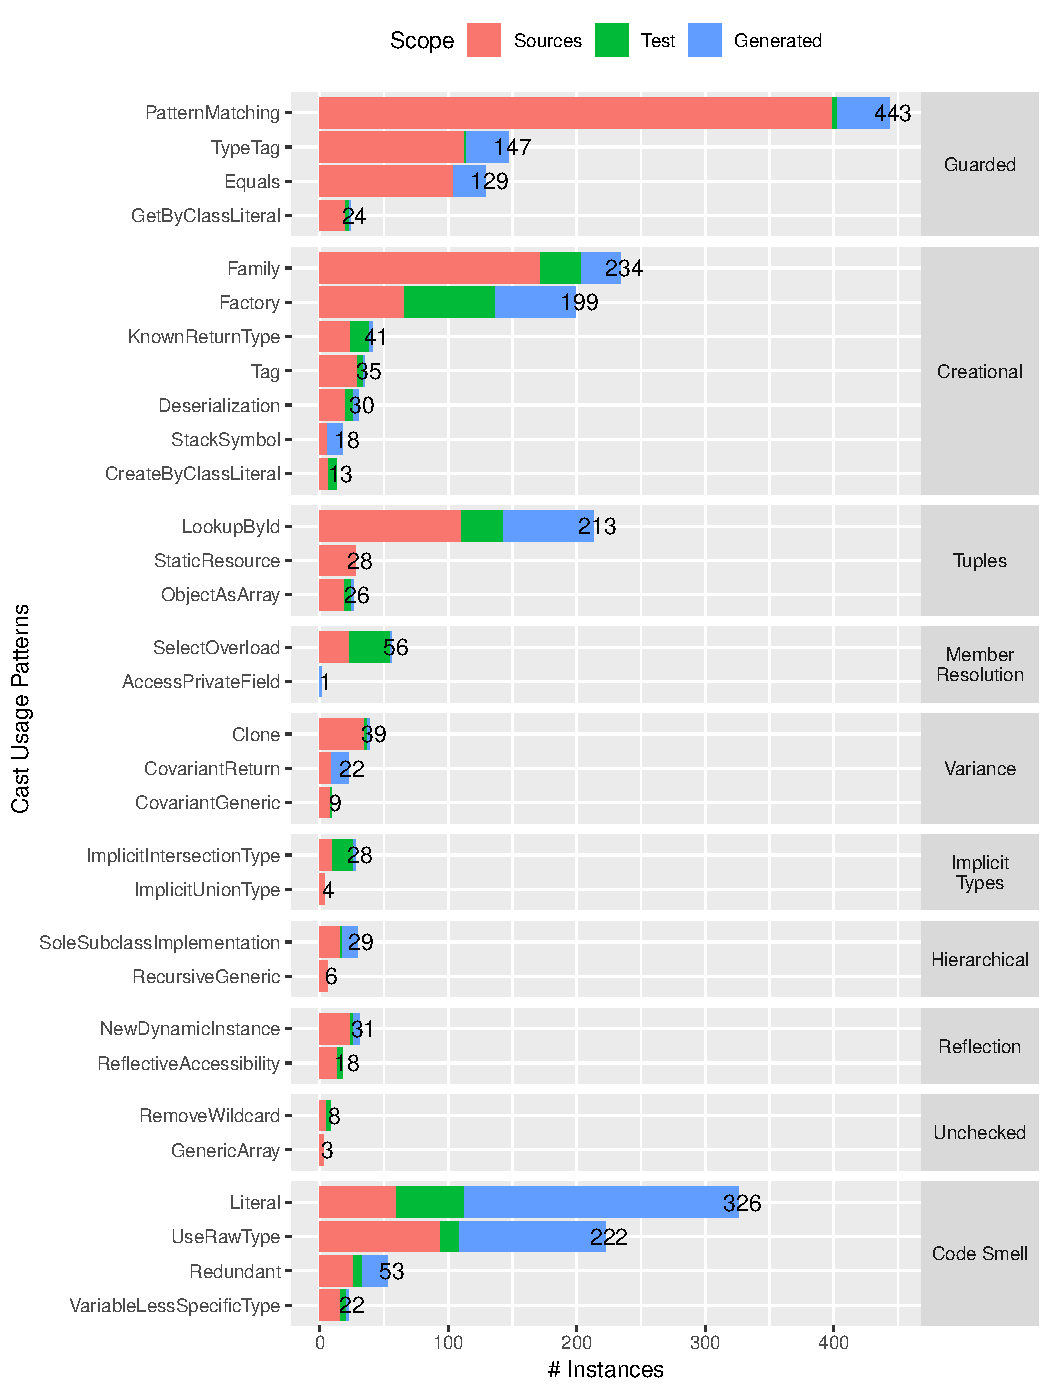
\includegraphics[width=\textwidth]{analysis/table-patterns-5000.pdf}
\caption{Cast Pattern Occurrences} \label{fig:patterns}
\end{figure}

\discuss{Matthias: Start a new subsection here.}
\todo{Matthias: When describing each pattern, you may want to repeat the number of occurrences within the description {\scriptsize (maybe as part of the section title, or just below)}}
Each pattern is described using the following template:

\begin{itemize}
\item \textbf{Description.}
Tells what the pattern is about.
It gives a general overview of the structure of the pattern.
\item \textbf{Instances.}
Gives one or more concrete examples found in real code.
%
\done{Nate: What's the orange (hightlight color) mean? The line with the cast being inspected. Explain here}
%
Each example contains a highlighted line which shows the cast instance being inspected.
Please notice that the snippets presented here were slightly
modified for formatting purposes.
Moreover, to facilitate some snippet presentations,
we remove irrelevant code and replace it with the
comment \code{// [...]}.
For each instance presented here, we provide the link to the source code repository in \lgtm{}.
We provide the link in case the reader wants to do further inspection
of the presented snippet.
%
\done{Nate: List project name too.}
%
Instead of presenting \lgtm{} long URLs,
we have used the URL shortening service
\href{https://bitly.com/}{\bitly} for easier reading.
%
\done{Luis: Links were customized to include the project names.}
%
Each \bitly{} link was customized to include the project name.
\item \textbf{Detection.}
Describes briefly how this pattern was detected in terms of the tags introduced in the previous section.
\item \textbf{Discussion.}
Presents suggestions, flaws, or comments about the pattern.
\item \textbf{Related Patterns.}
%
\done{Nate: Remove "?"}
%
How the pattern being described relates to other patterns.
\end{itemize}

\group{Guarded}

\done{Matthias: Say what it means to be guarded.}
The patterns in this category are guarded casts.
A guarded cast is a cast such that before the cast is applied,
some condition --- the \emph{guard} -- needs to be verified.
The condition to be verified guarantees that the cast will not fail at runtime (unless there is a bug in the application), \ie,
the cast will not throw a \code{ClassCastException}.
Some kind of guards ensure that the cast will not fail at the language-level,
while others only can guarantee it at the application-level.


\begin{pattern}{PatternMatching}
This pattern is composed of a guard (\code{instanceof}) followed by a
cast on known subtypes of the static type.
Often there is just one case and the default case, \ie,
\code{instanceof} fails, does a no-op or reports an error.
Another common approach is to have several cases,
usually one \emph{per} subtype.

\instances{}
The following listing shows an example of the \thisp{} pattern.%
\footnote{\url{http://bit.ly/2FzYYHq}}
In this example, there is only one case

% https://lgtm.com/projects/g/OpenMods/OpenBlocks/snapshot/dist-2040060754-1524814812150/files/build/sources/java/openblocks/common/tileentity/TileEntityImaginary.java?sort=name&dir=ASC&mode=heatmap#L268
\begin{minted}[highlightlines=3]{java}
Item item = helmet.getItem();
if (item instanceof ItemImaginationGlasses)
	return ((ItemImaginationGlasses)item).checkBlock(what, helmet, this);
\end{minted}

Double typecase example
\footnote{\url{http://bit.ly/2FDN9Rd}}

% https://lgtm.com/projects/g/bbossgroups/bboss/snapshot/dist-2025970729-1524814812150/files/bboss-util/src/org/frameworkset/util/ObjectUtils.java?sort=name&dir=ASC&mode=heatmap#L228
\begin{minted}[highlightlines=25]{java}
public static boolean nullSafeEquals(Object o1, Object o2) {
	if (o1 == o2) {
		return true;
	}
	if (o1 == null || o2 == null) {
		return false;
	}
	if (o1.equals(o2)) {
		return true;
	}
	if (o1.getClass().isArray() && o2.getClass().isArray()) {
		if (o1 instanceof Object[] && o2 instanceof Object[]) {
			return Arrays.equals((Object[]) o1, (Object[]) o2);
		}
		if (o1 instanceof boolean[] && o2 instanceof boolean[]) {
			return Arrays.equals((boolean[]) o1, (boolean[]) o2);
		}
		if (o1 instanceof byte[] && o2 instanceof byte[]) {
			return Arrays.equals((byte[]) o1, (byte[]) o2);
		}
		if (o1 instanceof char[] && o2 instanceof char[]) {
			return Arrays.equals((char[]) o1, (char[]) o2);
		}
		if (o1 instanceof double[] && o2 instanceof double[]) {
			return Arrays.equals((double[]) o1, (double[]) o2);
		}
		if (o1 instanceof float[] && o2 instanceof float[]) {
			return Arrays.equals((float[]) o1, (float[]) o2);
		}
		if (o1 instanceof int[] && o2 instanceof int[]) {
			return Arrays.equals((int[]) o1, (int[]) o2);
		}
		if (o1 instanceof long[] && o2 instanceof long[]) {
			return Arrays.equals((long[]) o1, (long[]) o2);
		}
		if (o1 instanceof short[] && o2 instanceof short[]) {
			return Arrays.equals((short[]) o1, (short[]) o2);
		}
	}
	return false;
}
\end{minted}


\detection{}
To detect this pattern, we look

\discussion{}
The \thisp{} pattern can be seen as an \adhoc{}
alternative to pattern matching.
This construct can be seen in several other languages, \eg,
\haskell{}, \scala{}, and \cs{}.
There is an ongoing proposal%
\footnote{\url{http://openjdk.java.net/jeps/305}} to add pattern
matching to the \java{} language.

As a workaround, alternatives to the \thisp{} pattern can be the
visitor pattern or polymorphism.
But in some cases, the chain of \code{instanceof}s is of boxed types.
Thus no polymorphism can be used.

% Maybe this should be called properly instanceof-guarded cast, to be more specific.
% This pattern checks whether a parameter in an overridden method has a more specific type.
% A cast to a variable guarded by an \code{instanceof}.
% A variable is \emph{guarded} by a condition when the condition controls
% that access to the variable, and there is no assignment after the
% condition and before the access to that variable.

The \thisp{} pattern consists of testing the runtime type of a variable against several related types.
Based on rule taken from:
It was taken from a \lgtm{} rule\footnote{\url{https://lgtm.com/rules/910065/}}.

It is a technique that allows a developer to take different actions according to the runtime type of an object.
Depending on the --- runtime --- type of an object, different cases, usually one for each type will follow.

\end{pattern}

\begin{pattern}{TypeTag}
%
\done{Matthias: Your first example doesn't have the tag in the *same* object, but passes it as a separate variable.}
%
A cast instance belonging to the \thisp{} pattern is guarded by an application-specific test instead of using an \code{instanceof} test.

\instances{}
The following example%
\footnote{\url{http://bit.ly/JesusFreke_smali_2Ho8bVL}}
shows an instance of the \thisp{} pattern.
The cast type of the parameter \code{reference} is determined by the value of the parameter \code{referenceType}.

%https://lgtm.com/projects/b/JesusFreke/smali/snapshot/dist-1306230039-1524814812150/files/dexlib2/src/main/java/org/jf/dexlib2/writer/InstructionWriter.java?sort=name&dir=ASC&mode=heatmap#L492
\begin{minted}[highlightlines=8]{java}
private int getReferenceIndex(int referenceType, Reference reference) {
    switch (referenceType) {
        case ReferenceType.FIELD:
            return fieldSection.getItemIndex((FieldRefKey) reference);
        case ReferenceType.METHOD:
            return methodSection.getItemIndex((MethodRefKey) reference);
        case ReferenceType.STRING:
            return stringSection.getItemIndex((StringRef) reference);
        case ReferenceType.TYPE:
            return typeSection.getItemIndex((TypeRef) reference);
        case ReferenceType.METHOD_PROTO:
            return protoSection.getItemIndex((ProtoRefKey) reference);
        default:
            throw new ExceptionWithContext(
                "Unknown reference type: %d",  referenceType);
    }
}
\end{minted}

In the next example,%
\footnote{\url{http://bit.ly/FenixEdu_fenixedu-academic_2SUNOUJ}}
instead of a \code{switch} statement,
an \code{if} statement is used to guard the cast (in line 6).

%https://lgtm.com/projects/g/FenixEdu/fenixedu-academic/snapshot/dist-29270029-1524814812150/files/src/main/java/org/fenixedu/academic/ui/renderers/student/curriculum/StudentCurricularPlanRenderer.java?sort=name&dir=ASC&mode=heatmap#L853
\begin{minted}[highlightlines=6]{java}
for (final IEnrolment enrolment : dismissal.getSourceIEnrolments()) {
    if (enrolment.isExternalEnrolment()) {
        generateExternalEnrolmentRow(mainTable, (ExternalEnrolment) enrolment,
                level + 1, true);
    } else {
        generateEnrolmentRow(mainTable, (Enrolment) enrolment,
                level + 1, false, true, true);
    }
}
\end{minted}

\done{Nate: Why is this not pattern matching?}
%
In the next case%
\footnote{\url{http://bit.ly/apache_poi_2FW5SXU}}
a type test is performed --- through a method call --- before actually applying the cast to the variable \code{props} (line 3).
Note that the type test is internally using the \code{instanceof} operator (line 8).
Although in this case the type test is using an \code{instanceof} operator,
it is not considered \nameref{pat:PatternMatching} because the \code{instanceof} is located in a method call.

%https://lgtm.com/projects/g/apache/poi/snapshot/dist-1790760597-1524814812150/files/src/ooxml/java/org/apache/poi/xslf/usermodel/XSLFPropertiesDelegate.java?sort=name&dir=ASC&mode=heatmap#L1367
\begin{minted}[highlightlines=3]{java}
@Override
public CTSolidColorFillProperties getSolidFill() {
    return isSetSolidFill() ? (CTSolidColorFillProperties)props : null;
}

@Override
public boolean isSetSolidFill() {
    return (props instanceof CTSolidColorFillProperties);
}
\end{minted}

In some cases, the type to be casted to is the same in every branch.
The following snippet%
\footnote{\url{http://bit.ly/loopj_android-async-http_2IpIULk}}
shows an instance of this case.
The cast is applied to the \code{message.obj} field to (line 13),
according to the value of the \code{message.what} field (line 1).
However, a similar cast is applied in the first branch (line 3).
In both branches \code{message.obj} is of type \code{Object[]},
but in the case of \code{FAILURE\_MESSAGE},
the array contains one more element (line 16).
This suggests that the \code{(Object[]) message.obj} array denotes two different objects,
but are not distinguishable from the type system perspective.

%https://lgtm.com/projects/g/loopj/android-async-http/snapshot/dist-1879340034-1549372228293/files/library/src/main/java/com/loopj/android/http/AsyncHttpResponseHandler.java?sort=name&dir=ASC&mode=heatmap#L359
\begin{minted}[highlightlines=13]{java}
switch (message.what) {
    case SUCCESS_MESSAGE:
        response = (Object[]) message.obj;
        if (response != null && response.length >= 3) {
            onSuccess((Integer) response[0], (Header[]) response[1],
                    (byte[]) response[2]);
        } else {
            AsyncHttpClient.log.e(LOG_TAG, 
                    "SUCCESS_MESSAGE didn't got enough params");
        }
        break;
    case FAILURE_MESSAGE:
        response = (Object[]) message.obj;
        if (response != null && response.length >= 4) {
            onFailure((Integer) response[0], (Header[]) response[1],
                    (byte[]) response[2], (Throwable) response[3]);
        } else {
            AsyncHttpClient.log.e(LOG_TAG,
                    "FAILURE_MESSAGE didn't got enough params");
        }
        break;
    // [...]
}
\end{minted}


\detection{}
The detection of this pattern is similar to the \nameref{pat:PatternMatching} detection, but instead of looking for an \code{instanceof} guarded cast, we look for an application-specific guard.
The guard needs to determine either the resulting type of the cast instance, or
the subsequent operations applied to the result of the cast instance if the types in every branch are the same.

\discussion{}
In some cases, the \thisp{} pattern can be replaced by \nameref{pat:PatternMatching}.
However, if the application-specific tag is a numeric value,
the \thisp{} could perform better than the \nameref{pat:PatternMatching} using \code{instanceof}.
Moreover, there are situation where the \thisp{} can not be avoid since the types to be casted to are the same.

\related{}
%
\done{Nate: PatternMatching}
This pattern is related to \nameref{pat:PatternMatching} since both denoted guarded casts.
The difference is that \thisp{} uses an application-specific test.
\nameref{pat:GetByClassLiteral} could be seen as a special case of \thisp{} where the tag is a class literal.

\end{pattern}
\begin{pattern}{Equals}
This pattern is a common pattern to implement the \code{equals} method (declared in \code{java.lang.Object}).
A cast expression is guarded by either an \code{instanceof} test or a \code{getClass} comparison (usually to the same target type as the cast);
in an \code{equals}%
\footnote{\url{https://docs.oracle.com/javase/8/docs/api/java/lang/Object.html\#equals-java.lang.Object-}} method implementation.
This is done to check if the argument has same type as the receiver
(\code{this} argument).

Notice that a cast in an \code{equals} method is needed because it
receives an \code{Object} as a parameter.

\instances{}
The following listing%
\footnote{\url{http://bit.ly/neo4j_neo4j_2vJw94J}}
shows an example of the \pname{} pattern.
In this case,
\code{instanceof} is used to guard for the same type as the receiver.

%https://lgtm.com/projects/g/neo4j/neo4j/snapshot/dist-15760049-1519892555006/files/community/kernel/src/main/java/org/neo4j/kernel/impl/api/CountsRecordState.java?sort=name&dir=ASC&mode=heatmap&excluded=false#L182
\begin{minted}[highlightlines=7]{java}
@Override
public boolean equals(Object obj) {
    if ( this == obj ) {
        return true;
    }
    if ( (obj instanceof Difference) ) {
        Difference that = (Difference) obj;
        return actualFirst == that.actualFirst
          && expectedFirst == that.expectedFirst
          && actualSecond == that.actualSecond 
          && expectedSecond == that.expectedSecond
          && key.equals( that.key );
    }
    return false;
}
\end{minted}

Alternatively, the following listing%
\footnote{\url{http://bit.ly/neo4j_neo4j_2vKP0MW}}
shows another example of the \thisp{} pattern.
But in this case,
a \code{getClass} comparison is used to guard for the same type as the receiver.

%https://lgtm.com/projects/g/neo4j/neo4j/snapshot/dist-15760049-1519892555006/files/community/bolt/src/main/java/org/neo4j/bolt/v1/messaging/infrastructure/ValuePath.java?sort=name&dir=ASC&mode=heatmap&excluded=false#L278
\begin{minted}[highlightlines=7]{java}
@Override
public boolean equals( Object o ) {
    if ( this == o ) return true;
    if ( o == null || getClass() != o.getClass() )
        return false;

    ValuePath that = (ValuePath) o;
    return nodes.equals(that.nodes) &&
        relationships.equals(that.relationships);
}
\end{minted}

In some situations, the type casted to is not same as the enclosing class.
Instead, the type casted to is the super class of the enclosing class.
The following example%
\footnote{\url{http://bit.ly/square_sqlbrite_2HmHMYE}}
shows this scenario.
This usually happens when the Google AutoValue library%
\footnote{\url{https://github.com/google/auto/tree/master/value}}
is used.
The AutoValue is a code generator for value classes.

%https://lgtm.com/projects/g/square/sqlbrite/snapshot/3a9916985485ba5922097fe59a18230500f02df4/files/sample/build/generated/source/apt/debug/com/example/sqlbrite/todo/ui/$AutoValue_ListsItem.java?sort=name&dir=ASC&mode=heatmap&showExcluded=false#L52
\begin{minted}[highlightlines=13]{java}
@AutoValue
abstract class ListsItem implements Parcelable {
    // [...]
}

abstract class $AutoValue_ListsItem extends ListsItem {
    @Override
    public boolean equals(Object o) {
      if (o == this) {
        return true;
      }
      if (o instanceof ListsItem) {
        ListsItem that = (ListsItem) o;
        return (this.id == that.id())
             && (this.name.equals(that.name()))
             && (this.itemCount == that.itemCount());
      }
      return false;
    }
}
\end{minted}

The following shows a non-trivial implementation of equals.
\footnote{\url{http://bit.ly/bndtools_bnd_2SM5pOw}}

%https://lgtm.com/projects/g/bndtools/bnd/snapshot/dist-930051-1524814812150/files/biz.aQute.bndlib/src/aQute/bnd/osgi/resource/CapReq.java?sort=name&dir=ASC&mode=heatmap#L73
\begin{minted}[highlightlines=12]{java}
@Override
public boolean equals(Object obj) {
    if (this == obj)
            return true;
    if (obj == null)
            return false;
    if (obj instanceof CapReq)
            return equalsNative((CapReq) obj);
    if ((mode == MODE.Capability) && (obj instanceof Capability))
            return equalsCap((Capability) obj);
    if ((mode == MODE.Requirement) && (obj instanceof Requirement))
            return equalsReq((Requirement) obj);
    return false;
}
\end{minted}

\detection{}
The detection query looks for a cast expression inside an \code{equals} method implementation.
Moreover, the cast needs to be guarded by either an \code{instanceof} test or a \code{getClass} comparison.
And the type being casted to needs to be either the same as the enclosing class or a superclass of it.

\discussion{}
The pattern for an \code{equals} method implementation is well-known.

We found out that, with respect to cast,
most \code{equals} methods are implemented with the same structure.
Maybe avoid boilerplate code by providing code generation,
%
\todo{Nate: \rust{} traits too. \code{\#[derive(Eq)]} }
%
like in \haskell{} (with \code{deriving}).

\cite{vaziriDeclarativeObjectIdentity2007} propose a declarative approach to avoid boilerplate code when implementing both the \code{equals} and \code{hashCode} methods.
They manually analyzed several applications, and found there are many issues while implementing \code{equals()} and \code{hashCode()} methods.
It would be interesting to check whether these issues happen in real application code.

There is an exploratory document%
\footnote{\url{http://cr.openjdk.java.net/\~briangoetz/amber/datum.html}}
by Brian Goetz --- \java{} Language Architect --- addressing these issues from a more general perspective.
It is definitely a starting point towards improving the \java{} language.

\related{}
This pattern can be seen as a special instance of the \nameref{pat:PatternMatching} pattern.
\end{pattern}
\begin{pattern}{GetByClassLiteral}
A cast is using an application-specific guard,
but the guard depends on a class literal.

\instances{}
The following example,%
\footnote{\url{http://bit.ly/elastic_elasticsearch_2SSgsFV}}
shows an instance of the \thisp{} pattern.
A cast is performed to the \code{field} variable (line 22),
based whether the runtime class of the variable is actually \code{Short.class}.

%https://lgtm.com/projects/g/elastic/elasticsearch/snapshot/dist-1916470085-1524814812150/files/server/src/main/java/org/elasticsearch/common/lucene/Lucene.java?sort=name&dir=ASC&mode=heatmap#L478
\begin{minted}[highlightlines=22]{java}
Class type = field.getClass();
if (type == String.class) {
    out.writeByte((byte) 1);
    out.writeString((String) field);
} else if (type == Integer.class) {
    out.writeByte((byte) 2);
    out.writeInt((Integer) field);
} else if (type == Long.class) {
    out.writeByte((byte) 3);
    out.writeLong((Long) field);
} else if (type == Float.class) {
    out.writeByte((byte) 4);
    out.writeFloat((Float) field);
} else if (type == Double.class) {
    out.writeByte((byte) 5);
    out.writeDouble((Double) field);
} else if (type == Byte.class) {
    out.writeByte((byte) 6);
    out.writeByte((Byte) field);
} else if (type == Short.class) {
    out.writeByte((byte) 7);
    out.writeShort((Short) field);
} else if (type == Boolean.class) {
    out.writeByte((byte) 8);
    out.writeBoolean((Boolean) field);
} else if (type == BytesRef.class) {
    out.writeByte((byte) 9);
    out.writeBytesRef((BytesRef) field);
} else {
    throw new IOException("Can't handle sort field value of type ["+type+"]");
}
\end{minted}

\detection{}

\discussion{}

\related{}

\end{pattern}

\group{Creational}

\todo{Matthias: In these paragraphs, can you also enumerate the patterns by name, so readers see what's coming?}
\todo{Matthias: ???}
These patterns create to how they are created.

\begin{pattern}{Family}
Family polymorphism.

\instances{}

\begin{minted}[highlightlines=1]{java}
\end{minted}

\detection{}

\discussion{}
\cite{ernstFamilyPolymorphism2001}

\related{}

\end{pattern}
\begin{pattern}{Factory}
\todo{Also Logger}
Creates an object based on some arguments either to the method call or constructor.
Since the arguments are known at compile-time, cast to the specific type.

\todo{Nate: Move to "Related Patterns"}
Cast factory method result to subtype (special case of family polymorphism).
Usually Logger.getLogger.

The method is declared to return URLConnection but can return a more specific type based on the URL string.
Cast to that.
We should generalize this pattern.
%
\todo{Nate: Create with type descriptor "Tag"}

\instances{}
\todo{Describe}
\footnote{\url{http://bit.ly/connect2id_oauth-2-0-sdk-with-_2HvRlUX}}

\footnote{\url{https://docs.oracle.com/javase/8/docs/api/java/security/KeyPair.html\#getPrivate()}}

%https://lgtm.com/projects/b/connect2id/oauth-2.0-sdk-with-openid-connect-extensions/snapshot/dist-1311020143-1524814812150/files/src/test/java/com/nimbusds/oauth2/sdk/jose/jwk/RemoteJWKSetTest.java?sort=name&dir=ASC&mode=heatmap#L242
\begin{minted}[highlightlines=10]{java}
KeyPairGenerator pairGen = KeyPairGenerator.getInstance("RSA");
pairGen.initialize(1024);
KeyPair keyPair = pairGen.generateKeyPair();
RSAKey rsaJWK1 = new RSAKey.Builder((RSAPublicKey) keyPair.getPublic())
        .privateKey((RSAPrivateKey) keyPair.getPrivate())
        .keyID("1")
        .build();
keyPair = pairGen.generateKeyPair();
RSAKey rsaJWK2 = new RSAKey.Builder((RSAPublicKey) keyPair.getPublic())
        .privateKey((RSAPrivateKey) keyPair.getPrivate())
        .keyID("2")
        .build();
\end{minted}

\done{Also URLOpenConnection.}
\footnote{\url{http://bit.ly/apache_hadoop_2E6KY6T}}

\footnote{\url{https://docs.oracle.com/javase/8/docs/api/java/net/URL.html\#openConnection--}}

%https://lgtm.com/projects/g/apache/hadoop/snapshot/dist-956730001-1524814812150/files/hadoop-yarn-project/hadoop-yarn/hadoop-yarn-server/hadoop-yarn-server-resourcemanager/src/test/java/org/apache/hadoop/yarn/server/resourcemanager/webapp/TestRMWebServicesHttpStaticUserPermissions.java?sort=name&dir=ASC&mode=heatmap#L138
\begin{minted}[highlightlines=2]{java}
URL url = new URL("http://localhost:8088/ws/v1/cluster/apps");
HttpURLConnection conn = (HttpURLConnection) url.openConnection();
\end{minted}

\detection{}

\discussion{}

\related{}

\end{pattern}
\begin{pattern}{KnownReturnType}
There are cases when a method's return type is less specific than the
actual return type value.
This is usually to hide implementation details.
Nevertheless, sometimes it is convenient for the developer to work
directly on the actual return type.
%
\done{Nate: KnownReturnType?}
%
This pattern is used to cast from the method's return type to
the \emph{known} actual return type.

\instances{}

\footnote{\url{http://bit.ly/apache_kylin_2SIjooO}}


%https://lgtm.com/projects/g/apache/kylin/snapshot/dist-45150010-1524814812150/files/storage-hbase/src/main/java/org/apache/kylin/storage/hbase/steps/HBaseMRSteps.java?sort=name&dir=ASC&mode=heatmap#L211
\begin{minted}[highlightlines=1]{java}
final List<CubeSegment> mergingSegments = ((CubeInstance) seg.getRealization())
            .getMergingSegments((CubeSegment) seg);

public class CubeSegment implements IBuildable, ISegment, Serializable {
    // [...]
    private CubeInstance cubeInstance;
    // [...]
    public IRealization getRealization() {
        return cubeInstance;
    }
}

public class CubeInstance
            extends RootPersistentEntity implements IRealization, IBuildable {
    // [...]
}
\end{minted}


\footnote{\url{http://bit.ly/eclipse_pdt_2Ekeu9v}}

%https://lgtm.com/projects/g/eclipse/pdt/snapshot/dist-19313119-1524814812150/files/plugins/org.eclipse.php.debug.core/src/org/eclipse/php/internal/debug/core/zend/communication/DebugConnection.java?sort=name&dir=ASC&mode=heatmap#L795
\begin{minted}[highlightlines=1]{java}
debugTarget = (PHPDebugTarget) createDebugTarget(this, launch, URL,
        requestPort, process, runWithDebug, stopAtFirstLine, project);

protected IDebugTarget createDebugTarget(DebugConnection thread,
        ILaunch launch, String url, int requestPort, PHPProcess process,
        boolean runWithDebug, boolean stopAtFirstLine, IProject project)
        throws CoreException {
    return new PHPDebugTarget(thread, launch, url, requestPort, process,
            runWithDebug, stopAtFirstLine, project);
}

public class PHPDebugTarget extends PHPDebugElement
        implements IPHPDebugTarget, IBreakpointManagerListener, IStepFilters {
}
\end{minted}

\footnote{\url{http://bit.ly/apache_activemq_2EnSivc}}

%https://lgtm.com/projects/g/apache/activemq/snapshot/dist-11730660-1524814812150/files/activemq-client/src/main/java/org/apache/activemq/ActiveMQConnectionFactory.java?sort=name&dir=ASC&mode=heatmap#L235
\begin{minted}[highlightlines=1]{java}
throw (IllegalArgumentException)
        new IllegalArgumentException("Invalid broker URI: " + brokerURL)
        .initCause(e);
\end{minted}


\todo{Also Logger}
Logger here
\footnote{\url{http://bit.ly/skylot_jadx_2HIoR9X}}

%https://lgtm.com/projects/g/skylot/jadx/snapshot/dist-41240110-1524814812150/files/jadx-gui/src/main/java/jadx/gui/utils/LogCollector.java?sort=name&dir=ASC&mode=heatmap#L22
\begin{minted}[highlightlines=1]{java}
Logger rootLogger = (Logger) LoggerFactory.getLogger(Logger.ROOT_LOGGER_NAME);
\end{minted}



\detection{}

\discussion{}

\related{}

\end{pattern}
\begin{pattern}{Tag}
Used 

\instances{}

\footnote{\url{http://bit.ly/2HUmGki}}

%https://lgtm.com/projects/g/UniTime/cpsolver/snapshot/dist-4860376-1524814812150/files/src/org/cpsolver/ifs/assignment/context/AssignmentContextHolderMap.java?sort=name&dir=ASC&mode=heatmap#L47
\begin{minted}[highlightlines=9]{java}
protected Map<Integer,AssignmentContext> iContexts =
                new HashMap<Integer, AssignmentContext>();

@Override
@SuppressWarnings("unchecked")
public <U extends AssignmentContext> U getAssignmentContext(
                Assignment<V, T> assignment,
                AssignmentContextReference<V, T, U> reference) {
    U context = (U) iContexts.get(reference.getIndex());
    if (context != null) return context;
    
    context = reference.getParent().createAssignmentContext(assignment);
    iContexts.put(reference.getIndex(), context);
    return context;
}
\end{minted}

\detection{}

\discussion{}

\related{}
Related to \nameref{pat:VariableLessSpecificType}.
\nameref{pat:LookupById}.

\end{pattern}
\begin{pattern}{Deserialization}
This pattern is used to deserialize an object at run-time.

\instances{}
The following example%
\footnote{\url{http://bit.ly/internetarchive_heritrix3_2SF4j7k}}
shows how the \thisp{} pattern is used to create objects from a file system (line 19).

%https://lgtm.com/projects/g/internetarchive/heritrix3/snapshot/dist-12140105-1524814812150/files/engine/src/test/java/org/archive/crawler/datamodel/CrawlURITest.java?sort=name&dir=ASC&mode=heatmap#L83
\begin{minted}[highlightlines=19]{java}
final public void testSerialization()
        throws IOException, ClassNotFoundException {
    File serialize = new File(getTmpDir(),
            this.getClass().getName() + ".serialize");
    try {
        FileOutputStream fos = new FileOutputStream(serialize);
        ObjectOutputStream oos = new ObjectOutputStream(fos);
        oos.writeObject(this.seed);
        oos.reset();
        oos.writeObject(this.seed);
        oos.reset();
        oos.writeObject(this.seed);
        oos.close();
        // Read in the object.
        FileInputStream fis = new FileInputStream(serialize);
        ObjectInputStream ois = new ObjectInputStream(fis);
        CrawlURI deserializedCuri = (CrawlURI)ois.readObject();
        deserializedCuri = (CrawlURI)ois.readObject();
        deserializedCuri = (CrawlURI)ois.readObject();
        assertEquals("Deserialized not equal to original",
                this.seed.toString(), deserializedCuri.toString());
        String host = this.seed.getUURI().getHost();
        assertTrue("Deserialized host not null",
                host != null && host.length() >= 0);
    } finally {
        serialize.delete();
    }
}
\end{minted}

\detection{}
This pattern is characterized for a cast to the \code{readObject} method on a \code{ObjectInputStream} object.

\discussion{}
From a language design perspective,
the \thisp{} pattern is one of the most difficult patterns to avoid.
It is difficult to avoid because a compiler cannot verify at compile-time that a certain byte stream can be deserialized into an object of a given type.

\related{}
Both this pattern and the \nameref{pat:NewDynamicInstance} pattern create objects by using reflection.
\nameref{pat:StaticResource}

\end{pattern}
\begin{pattern}{NewDynamicInstance}
%
\todo{Nate: Why not Creational?}
%
Dynamically creates an object or array by means of reflection.
The \code{newInstance} method family declared in the \code{Class},%
\footnote{\url{https://docs.oracle.com/javase/8/docs/api/java/lang/Class.html\#newInstance--}}
\code{Array}\footnote{\url{https://docs.oracle.com/javase/8/docs/api/java/lang/reflect/Array.html\#newInstance-java.lang.Class-int-}}\(^{,}\)
\footnote{\url{https://docs.oracle.com/javase/8/docs/api/java/lang/reflect/Array.html\#newInstance-java.lang.Class-int...-}}
and \code{Constructor}%
\footnote{\url{https://docs.oracle.com/javase/8/docs/api/java/lang/reflect/Constructor.html\#newInstance-java.lang.Object...-}}
classes creates an object or array dynamically by means of reflection, \ie, the type of object being created is not known at compile-time.
This pattern consists of casting the result of these methods to the appropriate target type.

\instances{}
The following example%
\footnote{\url{http://bit.ly/2HC3IPg}}
shows a cast to the \code{Class.newInstance()}
method.

%https://lgtm.com/projects/g/apache/hadoop/snapshot/6bedbef6c5f2d937a6cbc268300ce2a39609d06c/files/hadoop-hdfs-project/hadoop-hdfs/src/main/java/org/apache/hadoop/hdfs/server/namenode/FSNamesystem.java?sort=name\&dir=ASC\&mode=heatmap\&showExcluded=false#L1039
\begin{minted}[highlightlines=1]{java}
logger = (AuditLogger) Class.forName(className).newInstance();
\end{minted}

The following example%
\footnote{\url{http://bit.ly/2Hp5Hqc}}
shows how to dynamically create an array, using the \texttt{Array} class.

%https://lgtm.com/projects/g/neo4j/neo4j/snapshot/27aaa67633e4d26446e38125d04fbbd27f938b75/files/community/collections/src/main/java/org/neo4j/helpers/collection/Iterables.java?sort=name\&dir=ASC\&mode=heatmap\&showExcluded=false#L403
\begin{minted}[highlightlines=1]{java}
return list.toArray( (T[]) Array.newInstance( componentType, list.size()));
\end{minted}

Whenever a constructor other than the default constructor is needed,
the \code{newInstance} method declared in the \code{Constructor} class
should be used to select the appropriate constructor,
as shown in the following example.
\footnote{\url{http://bit.ly/2HsUgOo}}

%https://lgtm.com/projects/g/gradle/gradle/snapshot/209c3175e75af6ac30cb66c02eda15b0f8b6a616/files/subprojects/internal-integ-testing/src/main/groovy/org/gradle/integtests/fixtures/executer/OutputScrapingExecutionFailure.java?sort=name\&dir=ASC\&mode=heatmap\&showExcluded=false#L174
\begin{minted}[highlightlines=1]{java}
return (Exception) Class
                       .forName(className)
                       .getConstructor(String.class)
                       .newInstance(message);
\end{minted}

The following example%
\footnote{\url{http://bit.ly/2HC33xg}}
shows a guarded instance of the \thisp{} pattern.
This seems rather unusual, as this pattern is not guarded.

%https://lgtm.com/projects/g/alibaba/LuaViewSDK/snapshot/dist-2037250419-1524814812150/files/Android/LuaViewSDK/src/com/taobao/luaview/global/LuaViewManager.java?sort=name&dir=ASC&mode=heatmap#L373
\begin{minted}[highlightlines=6]{java}
private static List<String> getMapperMethodNames(final Class clazz) {
    try {
        if (clazz != null) {
            Object obj = clazz.newInstance();
            if (obj instanceof BaseMethodMapper) {
                return ((BaseMethodMapper) obj).getAllFunctionNames();
            }
        }
    } catch (Exception e) {
        e.printStackTrace();
    }
    return null;
}
\end{minted}

There are cases when the cast is not directly applied to the result of the \code{newInstance} method.
The following snippet shows such a case.%
\footnote{\url{http://bit.ly/2HJtXUn}}
The cast is used to convert from \code{Class<?>} to \code{Class<ConfigFactory>} (line 4).
The \code{newInstance} invocation then does not need a direct cast (line 8) given the definition of the \code{clazz} variable (line 2).
Nevertheless, the cast is unchecked, and a \code{checkcast} instruction is going to be emitted anyway for the result of the \code{newInstance} invocation.

%https://lgtm.com/projects/g/pac4j/pac4j/snapshot/dist-4840350-1524814812150/files/pac4j-core/src/main/java/org/pac4j/core/config/ConfigBuilder.java?sort=name&dir=ASC&mode=heatmap#L25
\begin{minted}[highlightlines=4]{java}
ClassLoader tccl = Thread.currentThread().getContextClassLoader();
final Class<ConfigFactory> clazz;
if (tccl == null) {
    clazz = (Class<ConfigFactory>) Class.forName(factoryName);
} else {
    clazz = (Class<ConfigFactory>) Class.forName(factoryName, true, tccl);
}
final ConfigFactory factory = clazz.newInstance();
\end{minted}


\detection{}
This detection query looks for casts,
where the expression being cast is a call site to methods mentioned above.

\discussion{}
The cast here is needed because of the dynamic essence of reflection.
This pattern is mostly unguarded, that is,
the application programmer knows what target type is being created.

The following two code snippets:

\begin{minted}{java}
Class<?> c = Class.forName("java.lang.String");
String pf = (String) c.newInstance();
\end{minted}

\begin{minted}{java}
Class<String> c = (Class<String>) Class.forName("java.lang.String");
String pf = c.newInstance();
\end{minted}

compile to the same bytecode below.

\begin{lstlisting}[style=bytecode]
ldc           #24    // String java.lang.String
invokestatic  #26    // Method java/lang/Class.forName
astore_1
aload_1
invokevirtual #32    // Method java/lang/Class.newInstance
checkcast     #36    // class java/lang/String
\end{lstlisting}

\related{}
Reflection.

\end{pattern}
\begin{pattern}{StackSymbol}

\instances{}

\footnote{\url{http://bit.ly/2HF6nrF}}

%https://lgtm.com/projects/g/fabioz/Pydev/snapshot/dist-20832102-1524814812150/files/plugins/org.python.pydev.parser/src/org/python/pydev/parser/grammar27/TreeBuilder27.java?sort=name&dir=ASC&mode=heatmap#L231
\begin{minted}[highlightlines=1]{java}
            case JJTASSERT_STMT:
                exprType msg = arity == 2 ? ((exprType) stack.popNode()) : null;
                test = (exprType) stack.popNode();
                return new Assert(test, msg);
\end{minted}

\detection{}

\discussion{}

\related{}

\end{pattern}
\begin{pattern}{CreateByClassLiteral}
    
\instances{}
\done{Nate: CreateByClassLiteral}
The following snippet\footnote{\url{http://bit.ly/apache_karaf_2HE55gE}} shows an instance of the \thisp{} pattern. 
Even if a test against a class literal (\code{AtomicInteger.class}) is used to determine a suitable cast for the parameter \code{value}.

%https://lgtm.com/projects/g/apache/karaf/snapshot/dist-13960098-1524814812150/files/shell/core/src/main/java/org/apache/karaf/shell/support/converter/DefaultConverter.java?sort=name&dir=ASC&mode=heatmap#L117
\begin{minted}[highlightlines=4]{java}
public Object convertToNumber(Number value, Class toType) throws Exception {
    toType = unwrap(toType);
    if (AtomicInteger.class == toType) {
        return new AtomicInteger((Integer)convertToNumber(value,Integer.class));
    } else if (AtomicLong.class == toType) {
        return new AtomicLong((Long) convertToNumber(value, Long.class));
    } else if (Integer.class == toType) {
        return value.intValue();
    } else if (Short.class == toType) {
        return value.shortValue();
    } else if (Long.class == toType) {
        return value.longValue();
    } else if (Float.class == toType) {
        return value.floatValue();
    } else if (Double.class == toType) {
        return value.doubleValue();
    } else if (Byte.class == toType) {
        return value.byteValue();
    } else if (BigInteger.class == toType) {
        return new BigInteger(value.toString());
    } else if (BigDecimal.class == toType) {
        return new BigDecimal(value.toString());
    } else {
        throw new Exception("Unable to convert number "+value+" to "+toType);
    }
}
\end{minted}


\detection{}

\discussion{}

\related{}

\end{pattern}
\begin{pattern}{Composite}
    
\instances{}

\footnote{\url{http://bit.ly/flyingsaucerproject_flyingsaucer_2N2nYbY}}

%https://lgtm.com/projects/g/flyingsaucerproject/flyingsaucer/snapshot/dist-26624048-1524814812150/files/flying-saucer-core/src/main/java/org/xhtmlrenderer/newtable/TableBox.java#L711
\begin{minted}[highlightlines=3]{java}
public class TableBox extends BlockBox {
    // [...]
    protected TableSectionBox sectionAbove(
            TableSectionBox section, boolean skipEmptySections) {
        TableSectionBox prevSection = (TableSectionBox)section.getPreviousSibling();
    }
}

public abstract class Box implements Styleable {
    // [...]
    public Box getPreviousSibling() {
        // [...]
    }
}


\end{minted}

\detection{}

\discussion{}

\related{}

\end{pattern}


\group{Tuples}

\todo{Nate: Why?}
Tuples patterns.

\begin{pattern}{LookupById}
This pattern is used to extract stashed values from a generic container.

Lookup an object by ID, tag or name and cast the result
(it is used often in Android code).
It accesses a collection that holds values of different types
(usually implemented as \code{Collection<Object>} or as \code{Map<K, Object>}).

\instances

%https://lgtm.com/projects/g/loopj/android-async-http/snapshot/dist-1879340034-1518514025554/files/library/src/main/java/com/loopj/android/http/AsyncHttpClient.java?sort=name&dir=ASC&mode=heatmap&excluded=false#L258

In the example shown in listing,
% \footnote{\url{d}},
the \texttt{getAttribute} method returns \texttt{Object}.
The variable \texttt{context} is of type \texttt{BasicHttpContext},
which is implemented with \texttt{HashMap}.

\lstset{language=java,label=orga7c88d3,caption={Example of the \pname{} pattern.},captionpos=b,numbers=none,style=java}
\begin{lstlisting}
AuthState authState =
        (AuthState) context.getAttribute(ClientContext.TARGET_AUTH_STATE);
\end{lstlisting}

\discussion{}
%
\todo{Cut/Move to future work.}
%
This pattern suggests heterogeneous dictionary.
Given our manual inspection,
we believe that all dictionary keys and resulting types are known at
compile-time, \ie, by the programmer.
%
\done{Nate: Replace "restriction" for "inexpressiveness"}
%
But in any case a cast is needed given the inexpressiveness of the type system.
As a complementary analysis,
it would be interesting to check whether all call sites to
\code{getAttribute} receives a constant (\code{final static} field).

Notice that this pattern is not guarded by an \code{instanceof}.
However, the cast involved does not fail at runtime.
This means that the source of the cast is known to the programmer.
This raises the following questions:
\begin{itemize}
\item \emph{What kind of analysis is needed to detect the source of the cast?}
\item \emph{Is worth to have it?}
\item \emph{Is better to change API?}
\item \emph{How other --- statically typed --- languages support this kind of idiom?}
\item \emph{Could generative programming a.k.a. templates solve this problem?}
\end{itemize}

\end{pattern}
\begin{pattern}{StaticResource}
%
\todo{Nate: Why not LookupById?}
%
A cast to a method access to \code{findViewById} or a method that reads a static resource.
This is a pattern seen when using the Android platform. 

\instances{}

\footnote{\url{http://bit.ly/2HGbrMq}}

%https://lgtm.com/projects/g/pwittchen/NetworkEvents/snapshot/dist-2032650416-1524814812150/files/example/src/main/java/com/github/pwittchen/networkevents/app/MainActivity.java?sort=name&dir=ASC&mode=heatmap#L65
\begin{minted}[highlightlines=6]{java}
@Override
protected void onCreate(Bundle savedInstanceState) {
    super.onCreate(savedInstanceState);
    setContentView(R.layout.activity_main);
    connectivityStatus = (TextView) findViewById(R.id.connectivity_status);
    mobileNetworkType = (TextView) findViewById(R.id.mobile_network_type);
    accessPoints = (ListView) findViewById(R.id.access_points);
    busWrapper = getOttoBusWrapper(new Bus());
    networkEvents = new NetworkEvents(getApplicationContext(), busWrapper)
        .enableInternetCheck()
        .enableWifiScan();
}
\end{minted}

\detection{}

\discussion{}
%
\todo{Nate: Could be determined at compile-time.}
%
These casts could be solved by using code generation,
or partial classes as in \csharp{}.

\end{pattern}
\begin{pattern}{ObjectAsArray}
In this pattern an array is used as an untyped object.
A cast is applied to a constant array slot, \eg, \code{(String) array[1]}.

\instances{}
The following example%
\footnote{\url{http://bit.ly/datanucleus_datanucleus-core_2S1L5Zf}}
shows an instance of the \thisp{} pattern.
A cast is performed to a constant array slot: \code{(BitSet)currentState[3]} in line 11.
Nevertheless, the \code{currentState} parameter is accessed in lines 7 and 15 with constant indices, denoting an untyped object.
Looking further, in the \code{else} branch (line 17) is where the array is being created matching the usage mentioned above.

%https://lgtm.com/projects/g/datanucleus/datanucleus-core/snapshot/dist-14100061-1524814812150/files/src/main/java/org/datanucleus/state/StateManagerImpl.java?sort=name&dir=ASC&mode=heatmap#L3324
\begin{minted}[highlightlines=11]{java}
public Object[] replacingDetachedState(Detachable pc, Object[] currentState) {
    if ((flags&FLAG_RESETTING_DETACHED_STATE) != 0) {
        return null;
    } else if ((flags&FLAG_RETRIEVING_DETACHED_STATE) != 0) {
        // Retrieving the detached state from the detached object
        // Don't need the id or version since they can't change
        BitSet theLoadedFields = (BitSet)currentState[2];
        for (int i = 0; i < this.loadedFields.length; i++) {
            this.loadedFields[i] = theLoadedFields.get(i);
        }
        BitSet theModifiedFields = (BitSet)currentState[3];
        for (int i = 0; i < dirtyFields.length; i++) {
            dirtyFields[i] = theModifiedFields.get(i);
        }
        setVersion(currentState[1]);
        return currentState;
    } else {
        // Updating the detached state in the detached object with our state
        Object[] state = new Object[4];
        state[0] = myID;
        state[1] = getVersion(myPC);
        // Loaded fields
        BitSet loadedState = new BitSet();
        for (int i = 0; i < loadedFields.length; i++) {
            if (loadedFields[i]) {
                loadedState.set(i);
            } else {
                loadedState.clear(i);
            }
        }
        state[2] = loadedState;
        // Modified fields
        BitSet modifiedState = new BitSet();
        for (int i = 0; i < dirtyFields.length; i++) {
            if (dirtyFields[i]) {
                modifiedState.set(i);
            } else {
                modifiedState.clear(i);
            }
        }
        state[3] = modifiedState;
        return state;
    }
}
\end{minted}

\detection{}

\discussion{}
%
\todo{Nate: Code Smell?}
%
This pattern usually suggests an abuse of the type system.

\related{}

\end{pattern}

\group{Member Resolution}

\begin{pattern}{SelectOverload}
This pattern is used to select
the appropriate version of an overloaded method%
\footnote{Using ad-hoc polymorphism~\cite{stracheyFundamentalConceptsProgramming2000}}
where two or more of its implementations differ \emph{only} in some argument type.

A cast to \code{null} is often used to select against different versions
of a method, \ie{}, to resolve method overloading ambiguity.
Whenever a \code{null} value needs to be an argument of an a cast is
needed to select the appropriate implementation.
This is because the type of \code{null} has the special type \emph{null}%
\footnote{\url{https://docs.oracle.com/javase/specs/jls/se8/html/jls-4.html\#jls-4.1}}
which can be treated as any reference type.
In this case,
the compiler cannot determine which method implementation to select.

\instances{}
The following listing%\footnote{\url{http://bit.ly/2FENovD}}
shows an example of \pname{} pattern.
In this example, there are three versions of the \code{onSuccess} method,
The cast \code{(String) null} is used to select the appropriate version
(line 7), based on the third parameter.
Overloaded methods that differ only in their argument type (the third one).

Another use case is to select the appropriate the right argument when
calling a method with variable arguments.

% https://lgtm.com/projects/g/loopj/android-async-http/snapshot/dist-1879340034-1518514025554/files/library/src/main/java/com/loopj/android/http/JsonHttpResponseHandler.java?sort=name\&dir=ASC\&mode=heatmap\&excluded=false#L150
\begin{minted}[highlightlines=1]{java}
onSuccess(statusCode, headers, (String) null);
\end{minted}

\begin{minted}{java}
public void onSuccess(
      int statusCode, Header[] headers, JSONObject response) {...}

public void onSuccess(
      int statusCode, Header[] headers, JSONArray response) {...}

public void onSuccess(
      int statusCode, Header[] headers, String responseString) {...}
\end{minted}

In the following example\footnote{\url{http://bit.ly/2FC9Llb}}
\code{actual.data()} returns \code{Long}.

% https://lgtm.com/projects/g/spullara/redis-protocol/snapshot/dist-41940059-1524814812150/files/client/src/test/java/redis/client/AllCommandsTest.java?sort=name&dir=ASC&mode=heatmap#L366
\begin{minted}[highlightlines=2]{java}
private void eq(long expected, IntegerReply actual) {
      assertEquals(expected, (long) actual.data());
}

public static void assertEquals(Object expected, Object actual) { }
public static void assertEquals(long expected, long actual) { }
\end{minted}


\footnote{\url{http://bit.ly/2HDAkbF}}

%https://lgtm.com/projects/g/groovy/groovy-core/snapshot/dist-45390050-1524814812150/files/src/main/org/codehaus/groovy/runtime/DefaultGroovyMethods.java?sort=name&dir=ASC&mode=heatmap#L6715
\begin{minted}[highlightlines=1]{java}
\end{minted}

\detection{}
Listing \ref{org9e0faf3} shows how to detect this pattern.
This pattern shows up when a cast is directly applied to the \texttt{null} constant.

\lstset{language=sql,label=org9e0faf3,caption={Detection of the \pname{} pattern.},captionpos=b,numbers=none,style=ql}
\begin{lstlisting}
import java

from CastExpr ce, NullLiteral nl
where ce.getExpr() = nl
select ce
\end{lstlisting}

\discussion{}
Casting the \code{null} constant seems rather artificial.
This pattern shows either a lack of expressiveness in \java{} or
a bad \api{} design.
Several other languages support default parameters, \eg{},
\scala{}, \csharp{} and \cpp{}.
Adding default parameters might be a partial solution.
% \todo{Relate null as theorical point of view in the TAPL book.}
\end{pattern}

\begin{pattern}{ReflectiveAccessibility}

This pattern accesses a field of an object by means of reflection.
It uses reflection because at compile time the field is unaccesible.
Usually the method \code{setAccessible(true)} is invoked on the field
before actually getting the value from an object.

\instances

%https://lgtm.com/projects/g/loopj/android-async-http/snapshot/dist-1879340034-1529316783166/files/library/src/main/java/com/loopj/android/http/AsyncHttpClient.java?sort=name&dir=ASC&mode=heatmap&showExcluded=false#L445

The following cast
% \footnote{\url{d}}
uses this pattern:

\begin{lstlisting}[style=java,caption=Using \code{Field::get} to gain access to a field.]
f.setAccessible(true);
HttpEntity wrapped = (HttpEntity) f.get(entity);
\end{lstlisting}

\end{pattern}

\begin{pattern}{AccessPrivateField}
Perform an upcast to access a private field defined within the same class.
Notice that there is only one instance of this pattern,
and from generated code.

\instances{}

\footnote{\url{http://bit.ly/FenixEdu_fenixedu-academic_2SQxlkC}}

%https://lgtm.com/projects/g/FenixEdu/fenixedu-academic/snapshot/dist-29270029-1524814812150/files/target/generated-test-sources/dml-maven-plugin/org/fenixedu/academic/domain/residence/StudentsPerformanceReport_Base.java?sort=name&dir=ASC&mode=heatmap#L12
\begin{minted}[highlightlines=4]{java}
public abstract class StudentsPerformanceReport_Base extends QueueJobWithFile {
    // [...]
    public ExecutionSemester getValue(StudentsPerformanceReport o1) {
        return ((StudentsPerformanceReport_Base)o1).executionSemester.get();
    }
    private OwnedVBox<ExecutionSemester> executionSemester;
}
 
public class StudentsPerformanceReport extends StudentsPerformanceReport_Base {
    // [...]
}
\end{minted}

\detection{}

\discussion{}

\related{}

\end{pattern}

\group{Variance}

\begin{pattern}{Clone}
A cast to a \code{clone} method.

\instances

\end{pattern}
\begin{pattern}{CovariantReturn}

\instances{}
CovariantReturn
\footnote{\url{http://bit.ly/apache_cayenne_2SMAdyV}}

%https://lgtm.com/projects/g/apache/cayenne/snapshot/dist-1890050-1524814812150/files/modeler/cayenne-modeler/src/main/java/org/apache/cayenne/modeler/undo/TextCompoundEdit.java?sort=name&dir=ASC&mode=heatmap#L74
\begin{minted}[highlightlines=1]{java}
EditorView editorView = ((CayenneModelerFrame) Application.
        getInstance().getFrameController().getView())
        .getView();
\end{minted}

\todo{Luis: Get bitly link.}
\footnote{\url{}}

%https://lgtm.com/projects/g/aws-amplify/aws-sdk-android/snapshot/dist-2970378-1524814812150/files/aws-android-sdk-autoscaling/src/main/java/com/amazonaws/services/autoscaling/model/transform/ResourceContentionExceptionUnmarshaller.java?sort=name&dir=ASC&mode=heatmap#L39
\begin{minted}[highlightlines=1]{java}
public class ResourceContentionExceptionUnmarshaller extends StandardErrorUnmarshaller {
    public ResourceContentionExceptionUnmarshaller() {
        super(ResourceContentionException.class);
    }
    public AmazonServiceException unmarshall(Node node) throws Exception {
        // Bail out if this isn't the right error code that this
        // marshaller understands.
        String errorCode = parseErrorCode(node);
        if (errorCode == null || !errorCode.equals("ResourceContention"))
            return null;
        ResourceContentionException e = (ResourceContentionException) super.unmarshall(node);
        return e;
    }
}

        
\end{minted}

\detection{}
    
\discussion{}
    
\related{} 

\end{pattern}{CovariantReturn}
\begin{pattern}{CovariantGeneric}
According to the generics are invariant.

\instances{}
The following snippet%
\footnote{\url{http://bit.ly/arpruss_raspberryjammod_2USL7Ai}}


\footnote{\url{https://docs.oracle.com/javase/8/docs/api/java/util/Collections.html\#singletonList-T-}}

%https://lgtm.com/projects/g/arpruss/raspberryjammod/snapshot/dist-1796220064-1524814812150/files/build/sources/java/org/java_websocket/drafts/Draft_10.java?sort=name&dir=ASC&mode=heatmap#L157
\begin{minted}[highlightlines=5]{java}
@Override
public List<Framedata> createFrames( String text, boolean mask ) {
    FrameBuilder curframe = new FramedataImpl1();
    // [...]
    return Collections.singletonList( (Framedata) curframe );
}

public interface FrameBuilder extends Framedata {
    // [...]
}

public class Collections {
    public static <T> List<T> singletonList(T o) {
        // [...]
    }
}
\end{minted}

The 
\footnote{\url{http://bit.ly/jfaster_mango_2EhXzUW}}

%https://lgtm.com/projects/g/jfaster/mango/snapshot/dist-1793930711-1524814812150/files/src/test/java/org/jfaster/mango/operator/UpdateOperatorTest.java?sort=name&dir=ASC&mode=heatmap#L125
\begin{minted}[highlightlines=6]{java}
@Test
public void testUpdateReturnBoolean() throws Exception {
    // [...]
    List<Object> args = boundSql.getArgs();
    // [...]
    assertThat(args.get(0), equalTo((Object) "ash"));
    // [...]
}

public static <T> Matcher<T> equalTo(T operand) {
    // [...]
}
\end{minted}


\footnote{\url{http://bit.ly/spockframework_spock_2UYEsF5}}

\footnote{\url{http://docs.groovy-lang.org/latest/html/api/org/codehaus/groovy/ast/expr/ArrayExpression.html\#<init>(org.codehaus.groovy.ast.ClassNode,java.util.List)}}

%https://lgtm.com/projects/g/spockframework/spock/snapshot/dist-7950040-1524814812150/files/spock-core/src/main/java/org/spockframework/compiler/WhereBlockRewriter.java?sort=name&dir=ASC&mode=heatmap#L360
\begin{minted}[highlightlines=5]{java}
dataProcessorStats.add(
    new ReturnStatement(
        new ArrayExpression(
            ClassHelper.OBJECT_TYPE,
            (List) dataProcessorVars)));

private final List<VariableExpression> dataProcessorVars = new ArrayList<>();

public class ArrayExpression extends Expression {
    public ArrayExpression(ClassNode elementType,
                       java.util.List<Expression> expressions) {}
}
\end{minted}


\footnote{\url{http://bit.ly/EngineHub_WorldGuard_2IVUOx1}}

%https://lgtm.com/projects/g/EngineHub/WorldGuard/snapshot/dist-1795351250-1524814812150/files/worldguard-legacy/src/test/java/com/sk89q/worldguard/protection/FlagValueCalculatorTest.java?sort=name&dir=ASC&mode=heatmap#L1024


\detection{}

\discussion{}

Avoided with
\code{Collections.<Framedata>singletonList(curframe)}
From \java{} 8 this cast is unnecesary due to better type inference.
\footnote{\url{https://docs.oracle.com/javase/specs/jls/se8/html/jls-18.html\#jls-18.5}}

\todo{Mention}
reference \cite{altidorTamingWildcardsCombining2011}

\related{}

\end{pattern}

\group{Implicit Types}

\begin{pattern}{ImplicitIntersectionType}
Cast a reference $v$ of type --- class or interface --- $T$ to an
interface type $I$ whether $T$ does not implement $I$.
The cast succeeds at runtime because all possible runtime types of $v$
actually implement the interface $I$.
For instance, in \code{(Comparable)(Number)4}, \code{Number} does not
implement the \code{Comparable} interface, but class \code{Integer} does.

\instances{}

\footnote{\url{http://bit.ly/senbox-org_snap-desktop_2FQOt4v}}

\begin{minted}[highlightlines=1]{java}
final Comparable max = (Comparable) properties.getMaxValue();
\end{minted}

Dynamic Proxy implementation
\footnote{\url{http://bit.ly/CloudSlang_cloud-slang_2EkgP4l}}

%https://lgtm.com/projects/g/CloudSlang/cloud-slang/snapshot/dist-13290023-1524814812150/files/cloudslang-entities/src/main/java/io/cloudslang/lang/entities/bindings/values/PyObjectValueProxyFactory.java?sort=name&dir=ASC&mode=heatmap#L51
\begin{minted}[highlightlines=1]{java}
PyObjectValueProxyClass proxyClass = getProxyClass(pyObject);
PyObjectValue pyObjectValue = (PyObjectValue) proxyClass.getConstructor()
        .newInstance(proxyClass.getParams());
((Proxy) pyObjectValue).setHandler(new PyObjectValueMethodHandler(content, sensitive, pyObject));
\end{minted}

\detection{}

\discussion{}

\related{}

\end{pattern}
\begin{pattern}{ImplicitUnionType}

\instances{}

\footnote{\url{http://bit.ly/groovy_groovy-core_2SGzK16}}

\code{invokeMethod(String name, Object args)}
\code{call(Object... args)}

%https://lgtm.com/projects/g/groovy/groovy-core/snapshot/dist-45390050-1524814812150/files/src/main/groovy/util/Expando.java?sort=name&dir=ASC&mode=heatmap#L103
\begin{minted}[highlightlines=12]{java}
public Object invokeMethod(String name, Object args) {
    try {
        return super.invokeMethod(name, args);
    }
    catch (GroovyRuntimeException e) {
        // br should get a "native" property match first. getProperty includes such fall-back logic
        Object value = this.getProperty(name);
        if (value instanceof Closure) {
            Closure closure = (Closure) value;
            closure = (Closure) closure.clone();
            closure.setDelegate(this);
            return closure.call((Object[]) args);
        } else {
            throw e;
        }
    }
}
\end{minted}

\detection{}

\discussion{}

\related{}

\end{pattern}

\group{Hierarchical}

\begin{pattern}{SoleSubclassImplementation}

\instances{}
The following example%
\footnote{\url{http://bit.ly/immutables_immutables_2S4BoJs}}

%https://lgtm.com/projects/g/immutables/immutables/snapshot/dist-43930039-1524814812150/files/value-processor/target/generated-sources/annotations/org/immutables/value/processor/encode/ImmutableEncodedElement.java?sort=name&dir=ASC&mode=heatmap#L1734
\begin{minted}{java}
public final EncodedElement.Builder addAllThrown( Iterable<? extends Type> elements) {
    this.thrown.addAll(elements);
    return (EncodedElement.Builder) this;
}
\end{minted}

\detection{}

\discussion{}

\related{}

\end{pattern}
\begin{pattern}{RecursiveGeneric}

\instances{}

\detection{}

\discussion{}

\related{}

\end{pattern}

\group{Unchecked}

\begin{pattern}{GenericArray}

\instances{}
The following snippet%
\footnote{\url{http://bit.ly/ppiastucki_recast4j_2EM7zWK}}

%https://lgtm.com/projects/g/ppiastucki/recast4j/snapshot/dist-4860452-1524814812150/files/detourtilecache/src/main/java/org/recast4j/detour/tilecache/AbstractTileLayersBuilder.java?sort=name&dir=ASC&mode=heatmap#L50
\begin{minted}[highlightlines=1]{java}
List<?>[][] partialResults = new List[th][tw];
partialResults[ty][tx] = build(tx, ty, order, cCompatibility);
layers.addAll((List<byte[]>) partialResults[y][x]);

protected abstract List<byte[]> build(int tx, int ty, ByteOrder order, boolean cCompatibility);

\end{minted}

\detection{}

\discussion{}

\related{}

\end{pattern}
\begin{pattern}{RemoveWildcard}

\instances{}

\footnote{\url{}}

\begin{minted}[highlightlines=1]{java}

\end{minted}

\detection{}

\discussion{}

\related{}

\end{pattern}

\begin{pattern}{UnoccupiedTypeParameter}

\instances{}

Either this fluent \api{}
\footnote{\url{http://bit.ly/vavr-io_vavr_2SMIfI2}}

%https://lgtm.com/projects/g/vavr-io/vavr/snapshot/dist-11000099-1524814812150/files/vavr/src/main/java/io/vavr/control/Either.java?sort=name&dir=ASC&mode=heatmap#L398
\begin{listing}[H]
\caption{Either fluent \api{}}
\begin{minted}[highlightlines=9]{java}
public interface Either<L, R> extends Value<R>, Serializable {
    // [...]
    @SuppressWarnings("unchecked")
    default <U> Either<U, R> mapLeft(Function<? super L, ? extends U> leftMapper) {
        Objects.requireNonNull(leftMapper, "leftMapper is null");
        if (isLeft()) {
            return Either.left(leftMapper.apply(getLeft()));
        } else {
            return (Either<U, R>) this;
        }
    }
    // [...]
}
\end{minted}
\end{listing}


\todo{Phantom Types, 2003, Cheney, Hinze}


\detection{}

\discussion{}

Discuss
\todo{Nate: Scala has a \code{Nothing} type}
\todo{Option[String] :> Option[Nothing]}

\related{}

\end{pattern}

\group{Code Smell}

These are code smells.

\begin{pattern}{Literal}
Cast a numeric literal or constant --- defined as \code{static final} ---
to a primitive type of
\code{byte}, \code{char}, \code{short}

\instances

The following listing shows an example of the \pname{Literal} pattern.%
\footnote{https://lgtm.com/projects/g/kaitoy/pcap4j/snapshot/dist-29675155-1524814812150/files/pcap4j-core/src/main/java/org/pcap4j/packet/namednumber/TcpPort.java?sort=name\&dir=ASC\&mode=heatmap\#L2329}

\begin{lstlisting}[style=java,caption=Literal example]
public static final TcpPort POWERBURST =
    new TcpPort((short)485, "Air Soft Power Burst");
\end{lstlisting}

\discussion

This pattern is related with \ref{pat:Prim}

\end{pattern}
\begin{pattern}{UseRawType}
When a generic method is not used as such.
The expression of this cast is a method invocation,
but the declaration differs from the usage.

\instances{}

Using a collection as a raw type.
\footnote{\url{http://bit.ly/2SD2HLm}}

%https://lgtm.com/projects/g/bcgit/bc-java/snapshot/dist-20740003-1524814812150/files/pkix/src/test/java/org/bouncycastle/cms/test/Rfc4134Test.java?sort=name&dir=ASC&mode=heatmap#L268
\begin{minted}[highlightlines=4]{java}
Collection c = recipients.getRecipients();
assertTrue(c.size() >= 1 && c.size() <= 2);
Iterator it = c.iterator();
verifyRecipient((RecipientInformation)it.next(), privKey);
\end{minted}

The following snippet\footnote{\url{http://bit.ly/2FAI5x5}}

\todo{Not necessarily mistakes, maybe requirement is jdk 1.2}

% https://lgtm.com/projects/g/robovm/robovm/snapshot/dist-39650108-1524814812150/files/rt/external/apache-xml/src/main/java/org/apache/xml/dtm/SecuritySupport12.java#L59
\begin{minted}[highlightlines=3]{java}
class SecuritySupport12 extends SecuritySupport {
    ClassLoader getSystemClassLoader() {
        return (ClassLoader)
            AccessController.doPrivileged(new PrivilegedAction() {
                public Object run() {
                    ClassLoader cl = null;
                    try {
                        cl = ClassLoader.getSystemClassLoader();
                    } catch (SecurityException ex) {}
                    return cl;
                }
            });
    }
}

public final class AccessController {
    // [...]
    public static <T> T doPrivileged(PrivilegedAction<T> action) {
        return action.run();
    }
    // [...]
}
\end{minted}

The following example%
\footnote{\url{http://bit.ly/2FSZKzm}}
uses the raw type of the \code{Comparable} --- generic --- interface.%
\footnote{\url{https://docs.oracle.com/javase/8/docs/api/java/lang/Comparable.html}}

%https://lgtm.com/projects/g/fangjie008/tiexue-mcp-parent/snapshot/dist-1505957596672-1524814812150/files/mcp-core/src/main/java/com/tiexue/mcp/core/dto/McpSettlementDetailDto.java?sort=name&dir=ASC&mode=heatmap#L100
\begin{minted}[highlightlines=6]{java}
public class McpSettlementDetailDto implements Comparable {
    // [...]

    @Override
    public int compareTo(Object o){
        McpSettlementDetailDto mcpSettlementDetailDto=(McpSettlementDetailDto)o;
        Integer newConsume=(int)mcpSettlementDetailDto.getConsume();
        Integer temp=((int)this.consume);
        return temp.compareTo(newConsume);
    }
}
\end{minted}




\detection{}

\discussion{}

\related{}

\end{pattern}
\begin{pattern}{Redundant}
    
A cast that is not necessary for compilation.

\instances
    
\end{pattern}
\begin{pattern}{VariableLessSpecificType}
This pattern occurs when a cast is applied to a variable (local variable,
parameter, or field),
that is usually being assigned once and
is declared with a less specific type than the type of the value 
that is being assigned to.
The type of the value being assigned to can be determined locally
either within the enclosing method or class.

\instances{}

* mention that other uses of uncompressedDirectBuf needs to be casted to.

The following example\footnote{\url{http://bit.ly/2FuDeO7}} shows the \thisp{} pattern.
We can see that the field \code{uncompressedDirectBuf} is being casted to the \code{java.nio.ByteBuffer} class (line $13$) but it is declared as \code{java.nio.Buffer} (line $3$).
Nevertheless, the field is assigned only once in the constructor (line $7$)
with a value of type \code{java.nio.ByteBuffer}.
The value assigned is returned by the method
\code{ByteBuffer.allocateDirect}.%
\footnote{\url{https://docs.oracle.com/javase/7/docs/api/java/nio/ByteBuffer.html\#allocateDirect(int)}}
Inspecting the enclosing class, there is no other assignment to the
field \code{uncompressedDirectBuf}.
Therefore, the cast pattern in line $13$ will always succeed.
Note that in this case the variable \code{uncompressedDirectBuf}
could have been declared as \code{final}.

% https://lgtm.com/projects/g/facebookarchive/hadoop-20/snapshot/dist-1802091768-1524814812150/files/src/core/org/apache/hadoop/io/compress/snappy/SnappyCompressor.java?sort=name&dir=ASC&mode=heatmap#L134
\begin{minted}[highlightlines=13]{java}
public class SnappyCompressor implements Compressor {
    // [...]
    private Buffer uncompressedDirectBuf = null;
    // [...]
    public SnappyCompressor(int directBufferSize) {
        // [...]
        uncompressedDirectBuf = ByteBuffer.allocateDirect(directBufferSize);
        // [...]
    }
    // [...]
    synchronized void setInputFromSavedData() {
        // [...]
        ((ByteBuffer) uncompressedDirectBuf).put(userBuf, userBufOff,
            uncompressedDirectBufLen);
        // [...]
    }
    // [...]
}
\end{minted}

\detection{}
To detect this pattern, a cast needs to be applied to a variable whose
value can be determined simply by looking at
the enclosing method or class.

\discussion{}
In most the cases this can be considered as a bad practice or
code smell.
This is because by only changing the declaration of the variable
to a more specific type type, the cast can be simply eliminated.

\related{}
This pattern is related to the \nameref{pat:Redundant} pattern.
Although \thisp{} is not redundant,
by only changing the declaration of the variable to a more specific type,
the cast becomes redundant.

\end{pattern}

\section{Discussion}\label{sec:casts:discussion}

\begin{table*}[t!]
\scriptsize
\centering
\caption{Categorization of Cast Usage Patterns}
\label{table:casts:categories}
\begin{tabularx}{\linewidth}{|r|X||c||c|c|c||c|}
\hdr \hline
    & \multicolumn{1}{|c||}{\textbf{Pattern}}
    & \textbf{Guarded?}
    & \textbf{Lang}
    & \textbf{Tools}
    & \textbf{Dev}
    & \textbf{Generic}
    \\ \hline
\row 1 & \nameref{pat:Typecase} & \cmark & \cmark & \cmark &  &  &  \\
\alt 2 & \nameref{pat:Stash} &  &  & \cmark &  &  &  \\
\row 3 & \nameref{pat:Factory} &  &  & \cmark &  &  &  \\
\alt 4 & \nameref{pat:Family} &  & \cmark &  &  &  &  \\
\row 5 & \nameref{pat:UseRawType} &  &  &  &  & \cmark & \cmark \\
\alt 6 & \nameref{pat:Equals} & \cmark &  &  & \cmark &  &  \\
\row 7 & \nameref{pat:KnownReturnType} &  &  & \cmark &  & \cmark &  \\
\alt 8 & \nameref{pat:Redundant} &  &  &  &  & \cmark &  \\
\row 9 & \nameref{pat:SelectOverload} &  & \cmark &  &  &  &  \\
\alt 10 & \nameref{pat:Deserialization} &  &  & \cmark &  &  &  \\
\row 11 & \nameref{pat:VariableSupertype} &  &  &  &  & \cmark &  \\
\alt 12 & \nameref{pat:NewDynamicInstance} &  &  & \cmark &  &  &  \\
\row 13 & \nameref{pat:SoleSubclassImplementation} &  & \cmark &  &  &  &  \\
\alt 14 & \nameref{pat:ObjectAsArray} &  &  &  &  & \cmark &  \\
\row 15 & \nameref{pat:ImplicitIntersectionType} &  & \cmark &  &  &  &  \\
\alt 16 & \nameref{pat:CovariantReturnType} &  & \cmark &  &  &  &  \\
\row 17 & \nameref{pat:RemoveWildcard} &  & \cmark &  &  &  & \cmark \\
\alt 18 & \nameref{pat:OperandStack} & \cmark & \cmark &  &  &  &  \\
\row 19 & \nameref{pat:ReflectiveAccessibility} &  & \cmark &  &  &  &  \\
\alt 20 & \nameref{pat:FluentAPI} &  & \cmark &  &  &  & \cmark \\
\row 21 & \nameref{pat:CovariantGeneric} &  & \cmark &  &  &  & \cmark \\
\alt 22 & \nameref{pat:Composite} &  & \cmark &  &  &  &  \\
\row 23 & \nameref{pat:GenericArray} &  & \cmark &  &  &  & \cmark \\
\alt 24 & \nameref{pat:AccessSuperclassField} &  &  &  &  & \cmark &  \\
\row 25 & \nameref{pat:UnoccupiedTypeParameter} &  & \cmark &  &  &  & \cmark \\

\hline
\end{tabularx}
\end{table*}

\newcommand{\gh}[1]{\emph{\textbf{#1}}}

There are common aspects shared by several patterns.
Table~\ref{table:casts:categories} presents a summary of the patterns and their different aspects.
The table consists of the following columns:
The \gh{Pattern} column indicates the name of the pattern.
\gh{Guarded?} The patterns here are guarded casts.
A guarded cast is a cast such that before the cast is applied,
some condition---the \emph{guard}---needs to be verified.
The condition to be verified guarantees that the cast will not fail at runtime (unless there is a bug in the application), \ie,
the cast will not throw a \code{ClassCastException}.
Some kind of guards ensure that the cast will not fail at the language-level,
while others only can guarantee it at the application-level.
\gh{Lang} These casts could be ameliorated if there is enough language support by changing the type system.
\gh{Analysis} The casts in this group could be checked with new analysis or compiler tools.
\gh{Auto} These casts are related to generated or boilerplate code.
\gh{Refactor} The casts with this aspect can be simply removed by the developer,
can be removed with little refactoring,
or suggest a code smell in the source code.
\gh{Generics} The casts in this category are related to generics or reified generics.

Many programming languages provide features to ameliorate the more common use cases of casts.
For instance,
\kotlin{}'s smart casts couple together the \code{instanceof} operator and cast operation on value, 
providing direct support for the \nameref{pat:Typecase} and \nameref{pat:Equals} patterns.
More generally, ML-style pattern matching subsumes this pattern.
Smart casts do not apply directly to the \nameref{pat:OperandStack} pattern,
since it is dispatched depending on some application-specific control state.
Other language features that might at least partially obviate the need for some of the patterns are
intersection types (\cf{} \nameref{pat:ImplicitIntersectionType}),
and self types or associated types (\cf{} 
\nameref{pat:Factory},
\nameref{pat:KnownReturnType},
\nameref{pat:Deserialization},
\nameref{pat:CovariantReturnType},
\nameref{pat:FluentAPI}).
Virtual classes~\citep{gbeta, scalaIndependentlyExtensible} and languages that support family polymorphism~\citep{ernstFamilyPolymorphism2001}
would help with casts in the \nameref{pat:Family} pattern.

Some cast can be automatically generated.
The \variant{StaticResource} variant in \nameref{pat:Stash} could be generated by a GUI editor,
given that it is most seen in Android applications.
The \nameref{pat:Equals} pattern is composed of boilerplate code.
For instance, \scala{}' solves this issue by introducing \emph{case classes},
which among other features, provide equality out of the box.

Our study also suggests analyses could be performed to improve code quality and eliminate some cast usages,
for instance finding opportunities to use generics instead (\cf{} \nameref{pat:UseRawType}),
removing redundant casts (\cf{} \nameref{pat:Redundant}),
or locating code smells (\cf{}
\nameref{pat:KnownReturnType},
\nameref{pat:VariableSupertype},
\nameref{pat:ObjectAsArray}).

Many cast patterns (\eg, 
\nameref{pat:RemoveWildcard},
\nameref{pat:GenericArray},
\nameref{pat:CovariantGeneric},
\nameref{pat:UnoccupiedTypeParameter})
are used either to 
workaround---or to take advantage of---the erasure of generic type parameters in \java{}.
Reified generics or definition-site, rather than use-site,
variance annotations~\citep{altidorTamingWildcardsCombining2011}
would reduce the need for these patterns.
There is an ongoing proposal%
\footnote{\url{https://openjdk.java.net/jeps/300}}~\citep{jep300}
to enhance \java{} with this feature.

\section{Conclusions}\label{sec:casts:conclusions}

The cast operator in \java{} bridges the gap between compile-time and run-time safety.
We have discovered several cast usage patterns.
We found the rationale behind some cast patterns is due to the inexpressiveness of \java{}'s type system.
On the other hand,
there are patterns that abuse or misuse it.

Many of the patterns we found should be unsurprising to most object-oriented programmers.
That nearly 45\% of casts are (possibly) unguarded 
suggests that developers use application-specific knowledge that cannot be easily encoded in
the type system to ensure the absence of run-time type errors.

Our study provides insight on the boundary between static and dynamic typing,
which may inform research on both static and dynamic,
as well as gradual type systems~\citep{Siek06gradualtyping}.
Conversely, this research can inform the design of extensions of the \java{} type system to reduce the need for casting.

